\documentclass[output=paper]{LSP/langsci}  
\author{Simon Pickl\affiliation{University of Salzburg, Department of German}} 
\title{Fuzzy dialect areas and prototype theory: {D}iscovering latent patterns in geolinguistic variation}
\abstract{In this article, a threefold link is established between the concept of dialect areas as scientific constructs, prototype theory as a descriptive model and factor analysis as an operationalisation of the former two. While the idea of using prototype theory to model emic, folk concepts of dialect areas is not new, it is here for the first time used to establish a scholarly, etic model of dialect areas, which will make it easier to compare emically and etically defined dialect areas in the future. Dialect areas can be conceived of as being crisp or fuzzy, but in most cases, they are best conceptualised as being fuzzy. Following work by Gaetano Berruto, fuzzy dialect areas are defined on the basis of sets of similarly distributed variants. In a second, more practical step, an operationalisation of this model is presented that uses factor analysis to extract spatial patterns from geolinguistic data that satisfy the model’s definition of dialect area. This methodology is illustrated by applying it to dialect data from Bavarian Swabia (Southern Germany). The geolinguistic structures revealed demonstrate the utility of factor analysis as a tool both for a detailed, in-depth differentiation of fuzzy dialect areas and for the detection of hitherto unknown, even very weak spatial patterns.

}

\maketitle 
\begin{document}

 
% \\
 
  
\section{Conceptualising dialect areas as fuzzy categories}

A priori, there is no such thing as a dialect area within a language space, i.e. the division of space in such areas is not a linguistic fact but an abstract concept that can differ depending on which definition is preferred and what criteria are chosen. Instead, language space can be conceived of as a dynamic arrangement of more or less mobile speakers, whose language behaviour allows linguistic forms to be attributed to certain places or regions. The distributions of these forms in the dimension of space do not normally constitute distinct dialect areas; more often, they form a spatial continuum. Any efforts to divide space into dialect areas are therefore acts of deliberation, and they will inevitably lead to different results depending on who performs them and on the approach taken. In that sense, dialect areas are constructions.

Being ideational rather than factual entities, they have a very long tradition as conceptual realities. In the history of dialectology, the existence of dialect areas has been a permanent presupposition since its very beginnings. The cognitive organisation of dialectal variation in terms of areas or varieties seems to be virtually inevitable, or at any rate very compelling, when dealing with language in space. This can be illustrated with a passage from \citet{chambers_dialectology_1998}, who state that they use such categories because they are handy, although they convey a strictly inaccurate picture of how language varieties are organised (in space or otherwise):

\begin{quote}
We shall […] be using labels for linguistic varieties that may suggest that we regard them as discrete entities. It will be as well, nevertheless, to bear in mind that this will in most cases be simply an ad hoc device and that the use of labels such as ‘language’, ‘dialect’ and ‘variety’ does not imply that continua are not involved.\\
\citep[12]{chambers_dialectology_1998}
\end{quote}

Also Peter \citet[807]{wiesinger_einteilung_1983} sees a general need or propensity to group similar ways of speaking together, which pertains to both linguists and non-linguists. Such groupings can be used, together with some salient linguistic features that are regarded as typical of them, to allocate speakers to a certain region. He stresses the practicality of regarding varieties as “discrete entities”, as doing so makes it easier for speakers and for linguists alike to deal with the complexity of dialectal differences. Put more generally, dialect areas or varieties can be regarded as the expression of a mental requirement for categories, the result of a conscious or unconscious attempt to cognitively organise a large number of disparate but interrelated ways of speaking. Dialect areas are, like all kinds of categories, groupings of elements that are defined by certain traits.

There are different kinds of categories; one basic distinction often made is between crisp and fuzzy categories. Crisp categories are defined by certain traits or features that are either necessary or sufficient conditions. These categories make it very easy to decide whether a given element belongs to them or not: if the element has all the necessary or at least one of the sufficient features, then it is a member of the category. However, the definition of categories and their conditions might be regarded as arbitrary in the first place. Fuzzy categories, on the other hand, are defined by a number of traits or features that serve as cues for that category, which are, however, neither necessary nor sufficient. If an element has many of the features associated with that category, then it is very likely that it belongs to it. Also the features themselves can have different degrees of importance for the category. Thus, no definitive answer is given as to whether an element belongs to a category or not; instead, membership is expressed as a gradual value or a probability. 

Dialect areas, like other kinds of categories, can be modelled as crisp or fuzzy categories. The classical dialect area with sharp boundaries is a crisp category of local dialects; \citet[108--113]{preston_applications_1993}, on the other hand, explicitly conceptualise dialect areas as “fuzzy sets”, assigning local membership values between 0 and 1 to individual dialects. To obtain crisp dialect areas, specific defining features have to be selected. In this way, it is almost inevitable to pick those features that will reconstruct and thereby justify preconceived notions of areas. Therefore it is preferable not to preselect defining features, but to look at a large set of variables which may or may not be relevant. Dialect areas can then be delimited by looking for sets of bundling isoglosses. Depending on whether they coincide exactly or bundle together loosely, they delimit crisp or fuzzy dialect areas. This method is well-established in dialectology (cf. e.g. Hans Kurath \citeyear{kurath_studies_1972}) and can be traced back to August \citet{bielenstein_grenzen_1892}. Craig M. Carver (1987) %MISSING REF
used a similar approach for constructing dialect ‘layers’ by combining features with similar geographic distribution. Also cluster analysis can be used to construct crisp or fuzzy dialect areas, depending on the method used (e.g. bootstrap clustering or noisy clustering; cf. \citealt[83]{nerbonne_gabmap_2011}), without having to preselect defining features. Generally, it seems advisable to use tools that allow for fuzzy structures to emerge from the data and do not restrict the form of the outcomes to crisp structures. Later on in this paper, I will argue that factor analysis is a statistical tool particularly suited for identifying fuzzy dialect areas.

From a more theoretical perspective, viewing dialects against the background of fuzzy set theory (cf. \citealt{zadeh_fuzzy_1965}) seems to provide a useful formalism for dealing with fuzzy dialect areas (cf. \citealt{preston_applications_1993}). Treating local dialects as elements that can have different degrees of belonging to an area implies that there are more and less \textsc{typical} examples of a dialect variety, which we could also call a \textsc{dialect type}. This way of treating dialects has also been used for describing how dialects are organised cognitively by members of the speech community.

\begin{quote}
Lectal categories, in short, constitute prototype categories. If lectal varieties constitute prototype categories, some realizations will be more ‘typical’ or ‘central’ or ‘better examples’ of a given variety than others. \citep[59]{kristiansen_style-shifting_2008}
\end{quote}

This is one example of a number of attempts to apply prototype theory to dialect geography, all of which are, as far as I see, folk linguistic approaches \citep{christen_dialekt_1998,anders_was_2010,klausmann_wie_2006,kristiansen_style-shifting_2008,beeching_prototype-theoretic_2009} in the sense that they deal with how speakers conceptualise language in space. Perceptual dialectology has produced many new insights in the cognitive perspective of language geography in the past decades, spearheaded by Dennis Preston (cf. e.g. \citealt{preston_perceptual_1989,preston_handbook_1999,anders_perceptual_2010}). It appears that prototype theory \citep{rosch_natural_1973,lakoff_women_1987} is a useful framework to describe how dialects are organised cognitively, and it is compatible with fuzzy set theory (see, however, \citealt[218--250]{kretzschmar_linguistics_2009}, who is critical of using prototype theory and favours schema theory). Prototype theory assumes that cognitive concepts are fundamentally fuzzy: examples for a concept can be more or less typical, depending on their traits or features (cf. also \citealt{bailey_boundaries_1973}). Consequently, a specific way of speaking can be a more or less typical example of a dialect type. Folk linguistic dialect types are \textsc{emic} categories; they are cognitive concepts of the speakers whose speech is at the same time the object of linguistic investigation.

There is no reason why the fundamental linguistic concept of a dialect variety should differ from the folk linguistic concept. In other words, scholarly or \textsc{etic} ideas about geolinguistic entities can and should have the same principal structure as lay persons’ implicit ideas about dialects in space while being based on transparent – and, as far as possible, objective – criteria that are not derived from the speakers’ ideas, but from scientific reasoning. Only in this way, the question of to what extent emic and etic dialect types coincide and why (not) can be tackled: In what way do some folk linguistic ideas of space diverge from linguistic ones, and why? It appears worthwhile to use a linguistic (etic) notion of dialect types that is similar to the folk linguistic (emic) one, but based on intersubjective criteria. This way, it becomes possible to compare emic and etic dialect types directly and identify how and why they differ. 

If dialect varieties – emic or etic ones – take the shape of fuzzy categories, then they have no clear-cut boundaries or distinct features; instead, their spatial distributions are fuzzy, and local dialects are typical of them to varying degrees. Also, linguistic features are not simply features of one variety or the other, but they have different degrees of relevance for them. Thus, individual dialects can be better or worse examples of a variety, i.e. they have different values of \textsc{typicality} for a dialect type. Typicality is a measure for the graded membership of dialects, thus providing the structure of a fuzzy set. If typicality or membership values of a dialect type are projected into space, the result is a graded or fuzzy dialect area; being fuzzy, it can overlap with other dialect areas. Linguistic features, on the other hand, can be better or worse cues for a dialect type, i.e. they have varying degrees of cue validity or \textsc{feature validity}. Consequently, the way in which dialect types are arranged in space takes the form of concretions with broad transition areas (cf. Figure~1). Note that there is no requirement for dialect types to have a core area in the sense that there must be locations that belong a hundred percent to them; instead, the core area of a dialect type can be defined as the area where it is \textsc{dominant}, i.e. the area where it is the dialect type with the highest local typicalities. There may even be dialect types that are dominant nowhere. Because dialect types overlap in space, they appear layered; the individual layers consist of congruent distribution areas of co-occurring linguistic forms.

\begin{figure}
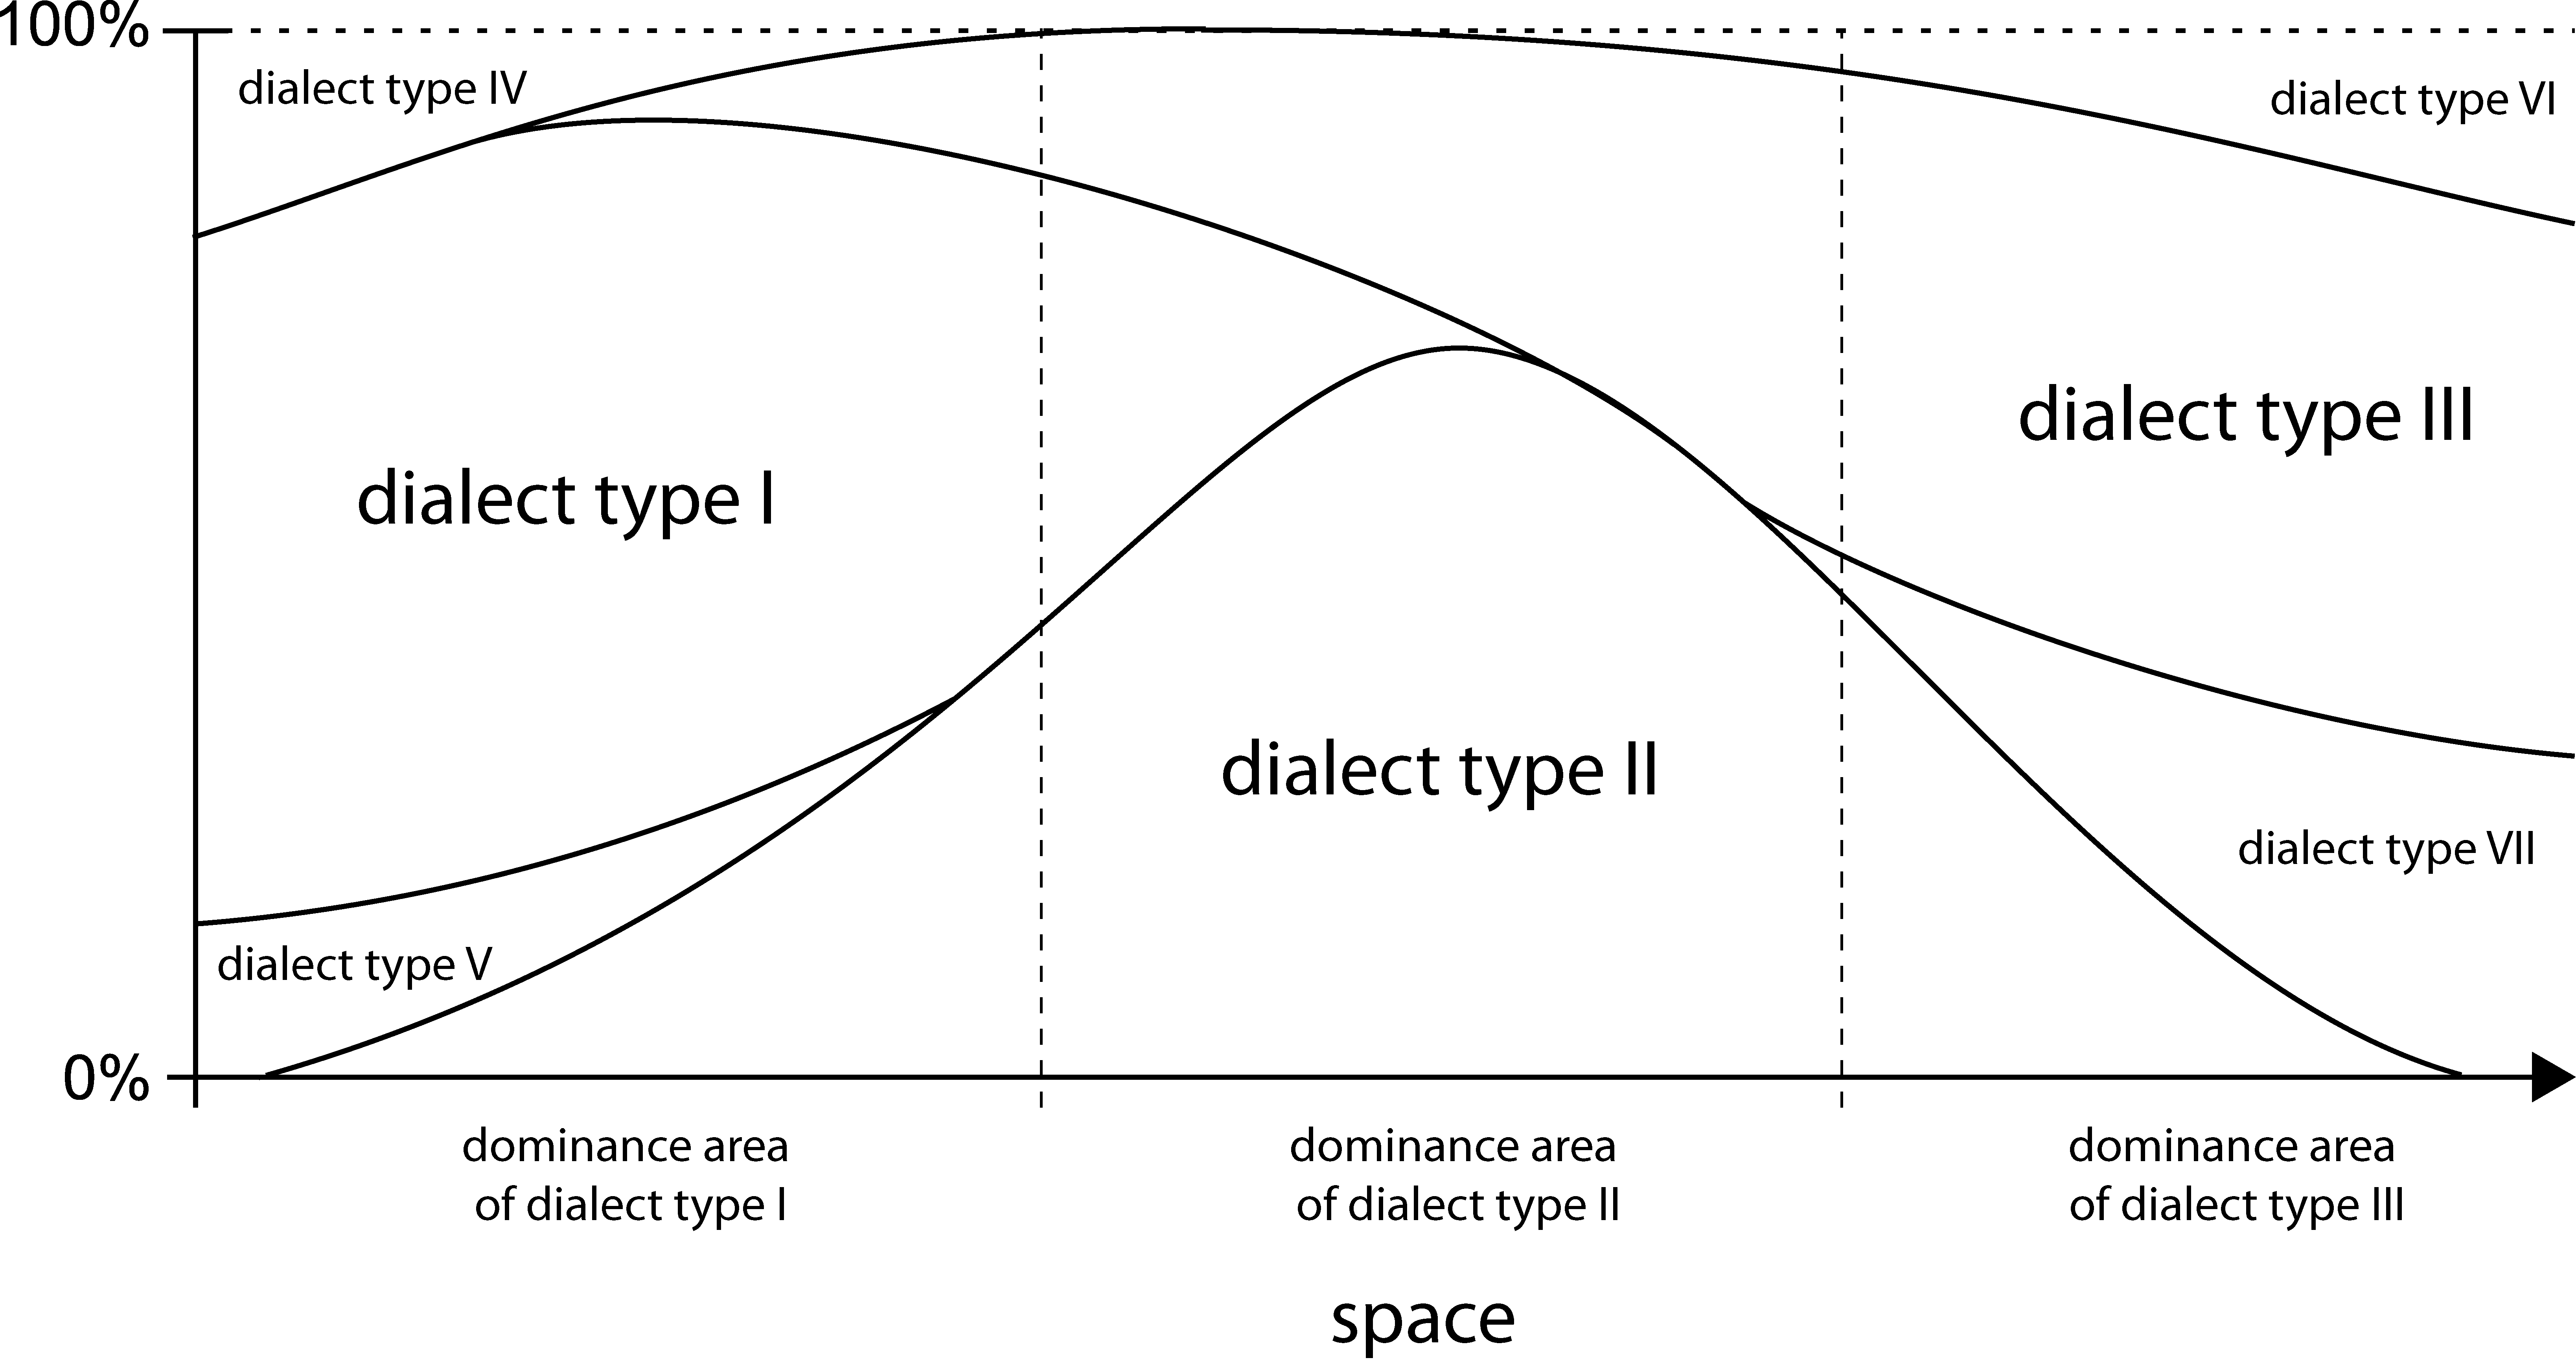
\includegraphics[width=\textwidth]{illustrations/pickl_fig1}
\caption{Layer model of dialect types in space.}
\label{fig:1}
\end{figure}

This is in line with Gaetano Berruto’s definition of varieties, which is based on the simple assumption that when a number of linguistic variants tend to occur together, then these variants constitute a variety:

\begin{quote}
The tendential co-occurrence of variants gives rise to linguistic varieties. Therefore, a linguistic variety is conceivable as a set of co-occurring variants; it is identified simultaneously by both such a co-occurrence of variants, from the linguistic viewpoint, and the co-occurrence of these variants with extralinguistic, social features, from the external, societal viewpoint.\\
\citep[229]{auer_identifying_2010}
\end{quote}

This notion captures several of the usual requirements for varieties: their relative internal homogeneity and their relative mutual dissimilarity, and also their association with language-external factors.\footnote{   It does not capture, however, their emic status, as required by \citet[99]{auer_konversationelle_1986} and \citet[389--390]{lenz_struktur_2003}. As I treat emic and etic varieties separately, focussing on etic varieties, this is consistent and does not pose a problem.} Varieties are thus condensations of co-occurring variants that can be pinned to a certain geographical expanse only to some extent – they are fuzzy and they overlap. Their arrangement in space is similar to the one depicted in Figure~1. According to Berruto, a variety as a condensation area is defined by certain co-occurring linguistic variants (its features). Depending on how many of these features are present in a given dialect, this dialect has a specific degree of membership between 0 (none of the features are present) and 1 (all of the features are present).

How are dialect types to be determined? Any method that is intended to identify linguistic varieties in the sense of Berruto’s condensations will have to identify co-occurrences among linguistic variants. Craig M. Carver’s (1987) %NO REF
approach did something similar in using lexical congruencies to establish ‘layers’ in American dialects,\footnote{I would like to thank an anonymous referee for making me aware of this connection.} “essentially speech areas characterized by sets of words with a similar geographic distribution” \citep[24]{boberg_north_2005}. The resulting structure is quite similar to what is illustrated in Figure~1. 

The remaining part of this paper is dedicated to demonstrating how the theoretical idea of fuzzy dialect types can be implemented methodologically and practically. It is to be shown that taking such an approach does not only reproduce well-established geolinguistic structures in a more nuanced way, but also that it yields new insights, e.g. regarding weaker, non-dominant structures.

\section{A tool for identifying dialect types}
There are various methods available for the identification of dialect areas (see \citealt{grieve_comparison_2014} for a more detailed comparison of popular statistical methods). Some of them, like fuzzy clustering, are suitable for identifying dialect types as fuzzy categories. However, I will argue that most of them are not suited for the identification of dialect types conceived of as layers of linguistic co-occurrence, either because of the structure of their outcomes or because of their internal working mechanisms, and that there are two options that are similarly well suited for this goal.

Cluster analysis, the quantitative method that is to date the most popular tool to identify dialect areas (see e.g. \citealt[17--29]{goebl_stammbaum_1983,prokic_recognizing_2008,prokic_families_2010}), analyses the aggregated similarities between local dialects to establish groups of local dialects that are relatively homogeneous internally and at the same time relatively distinct from each other. These groups or clusters are based on a measure of similarity between sites but not between distribution areas; it does not take into account the distribution patterns of individual variants and \textit{their} mutual similarities, which would be a requirement for identifying condensations in Berruto’s sense. Cluster analysis does not identify types and their features, but clusters. For this reason, it is also impossible for a cluster analysis to come up with anything more subtle than global, exclusively dominant areas; subordinate, non-dominant areas that are determined by smaller numbers of features cannot be identified by cluster analysis. So, even though there are ‘fuzzy’ implementations of cluster analysis that yield overlapping clusters (e.g. bootstrap clustering or noisy clustering; cf. \citealt{nerbonne_gabmap_2011}: 83), it is not a candidate for the operationalisation of dialect types. Bipartite spectral graph partitioning, which can also determine clusters of local dialects, simultaneously identifies the linguistic variants associated with these clusters (cf. \citealt{wieling_bipartite_2011}) and is therefore in theory suitable for identifying areas together with their features. However, for our purpose this method has the disadvantage that it does not yield fuzzy areas but crisp clusters, at least as implemented by \citet{wieling_bipartite_2011} or \citet{wieling_analyzing_2013}. 

Multi-dimensional scaling (MDS) (see \citealt[245]{wieling_advances_2015} for an overview), “the de facto standard in dialectometry” according to an anonymous referee, arranges local dialects in a coordinate system of two or more dimensions, thus summarising the multiple similarities between local dialects. Again, the basis for the analysis are the linguistic similarities between sites, not the similarities between distribution areas. “MDS takes a site × site distance table as input and tries to assign the sites in the table to coordinates in a small-dimensional space, typically consisting of two or three dimensions” \citep[245]{wieling_advances_2015}. Thus, it does not actually yield dialect areas but rather a dialect continuum without distinguishing condensations. Even if we took the axes as representing some sort of types, there would still be the problem, as with cluster analysis, that the results are based on global similarities between sites only, while similarities or differences between linguistic variants’ spatial distributions are not taken into account. Therefore, the results of MDS cannot be interpreted as dialect types as discussed in the preceding section.

Two methods that are similar in the form of their results, but not in their internal functioning, are promising candidates for identifying fuzzy dialect areas as dialect types. Both Principal Component Analysis (PCA) and Factor Analysis (FA)\footnote{For a general introduction to both methods, see \citet{tabachnick_using_2012}.} take feature × site matrices as data input and express recurring patterns in the data as principal components or \textsc{factors}, usually producing a principal component/factor × site matrix as output. Additionally, a principal component/factor × linguistic feature matrix can be calculated. One of the earliest applications of PCA/FA in linguistics comes from Douglas Biber, who used it to analyse stylistic variation in written texts.

\begin{quote}
In a factor analysis, a large number of original variables, in this case the frequencies of linguistic features, are reduced to a small set of derived variables, the `factors'. Each factor represents some area in the original data that can be summarized or generalized. That is, each factor represents an area of high shared variance in the data, a grouping of linguistic features that co-occur with a high frequency. \citep[79]{biber_variation_1988}
\end{quote}

As a method for the reduction of high-dimensionality data, FA condenses the variation in a large data collection to a smaller number of underlying tendencies or factors. PCA does something very similar. By summarising large numbers of variants that have similar distributions, the variation in a data collection is condensed, providing a summary of predominant patterns in the data. Thus factors – “grouping[s] of linguistic features that co-occur with a high frequency” – or principal components are exactly what an operationalised method for identifying dialect types as condensations of co-occurring variants in the geographical dimension should output. The principal components or factors can be seen as condensations or layers because they are summaries of the distributions of co-occurring variants. Since co-occurrence is mathematically determined in terms of correlations, it is a technical requirement that the variant occurrences are given in the form of something like frequencies. Thus both PCA and FA meet the requirements of identifying linguistic layers as condensations of co-occurring variants and of yielding fuzzy areas as results. Hence, applying FA or PCA to geolinguistic data to find spatial patterns that qualify as varieties seems promising.

PCA and FA work quite similarly as far as their outcomes are concerned, but they function differently ‘under the hood’. Both methods have been used several times before in dialectology.\footnote{See, among others, \citealt{shackleton_english-american_2005}; \citealt{hyvonen_multivariate_2007}; \citealt{szmrecsanyi_holistic_2011}; \citealt{wieling_analyzing_2013} for PCA and e.g. \citealt{clopper_north_2006}; \citealt{nerbonne_identifying_2006}; \citealt{grieve_statistical_2011} for FA. \citealt{grieve_corpus-based_2009} and \citealt{leinonen_acoustic_2010} use both, while \citealt{leino_comparison_2008} compare PCA and FA with other component models. The approach and data used in this paper are based on previous research by \citet{pickl_probabilistische_2013, pickl_verdichtungen_2013,buhler_dialektraume_2014,elmentaler_latente_2015} and \citet{proll_raumvariation_2015}.} For the present purpose, FA is favoured over PCA because FA is less susceptible to random variation and therefore “a more suitable method for identifying co-occurring linguistic features” \citep[106]{leinonen_acoustic_2010}. Leino \& Hyvönen, comparing different component models including FA and PCA in an application to Finnish data, found that FA “gave solid and easily interpretable results” (\citeyear[186]{leino_comparison_2008}) and could be used as a default method.

The implementation of FA for dialectometric analyses presented in the following section was developed in the DFG-funded research project \textit{New Dialectometry Using Methods of Stochastic Image Analysis}\footnote{   \textit{Neue Dialektometrie mit Methoden der stochastischen Bildanalyse} \\
(\url{http://www.philhist.uni-augsburg.de/de/lehrstuehle/germanistik/sprachwissenschaft/projekte/dialektometrie/})} (Department of German Linguistics, University of Augsburg, and Institute of Stochastics, Ulm University). It is included in \textit{GeoLing – a software package for geolinguistic data}, which was developed in the project and is available as open source software (GPLv3) at www.geoling.net. The results reported in this article were obtained using this software.

\section{Dialect types in Bavarian Swabia}

In this section, the approach outlined in the previous sections will be exemplified with data from the \textit{Sprachatlas von Bayerisch-Schwaben} (SBS, \citealt{konig_sprachatlas_1996}), a dialect atlas that covers an area in the south of Germany. The area of investigation is delimited by the administrative region of Swabia in the south-west of Bavaria plus some adjoining stretches in the north and east, minus a part in the south that is already covered by the \textit{Vorarlberger Sprachatlas} (VALTS). The data were collected under the direction of Werner König in the form of dialect interviews that were conducted at 272 record locations. The published version of the SBS contains approx. 2,700 maps covering lexical, morphological and phonetic variables in 14 volumes. Per location and map, up to three different variants are documented.

In previous research from the project that reported results from FA(\cite{pickl_probabilistische_2013,pickl_verdichtungen_2013,buhler_dialektraume_2014,proll_raumvariation_2015,proll_raumvariation_2015}), the individual subsets (lexicon, morphology, phonetics) were analysed either separately or all combined. In this article, the morphological and phonetic subsets will be analysed together, excluding the lexical subset to provide an additional angle. The rationale behind this is that morphology and phonetics are usually seen to be more systematically organised and thus more relevant for geolinguistic abstractions (cf. Francis 1983: 20%MISSING REF
; \citealt[41, 119]{labov_atlas_2006-1}).\footnote{For a complementary analysis, looking at the lexicon alone, see \citet{pickl_probabilistische_2013,pickl_verdichtungen_2013}; for an integrated analysis, looking at all linguistic subsets together, see \citet{proll_raumvariation_2015}.} For a more detailed comparison for FA based on different subsets, see \citet[84--132]{proll_raumvariation_2015}; generally, he finds that morphological and phonetic variation can be slightly better summarised (61~\% and 64 \% explained variance, respectively) than lexical variation (57~\% explained variance).

The data for this study consist of 831 phonetic and 541 morphological maps (1,372 in total) containing data from 272 locations. There are a total of 14,825 linguistic variants in the data,\footnote{The exact number of variants depends, of course, on the granularity of the classification of the records. For the SBS data, three levels of granularity have been defined, each being more general than the one before, thus aggregating more records together (cf. \citealt[75--78]{pickl_probabilistische_2013}; \citealt[47--48]{proll_raumvariation_2015}). For the analysis, I use Level 1 with the finest granularity, which means most of the differences between records are rendered as different variants.} i.e. each of the maps, representing an individual linguistic variable, contains on average 10.8 variants. In order to be workable for FA, these data have to be pre-processed. This is done by converting their occurrences at each location into ‘weights’ ranging between 0 and 1; the weight is the fraction of times a variant has been recorded at a location in relation to all records of variants at that location. Thus 0 means that a variant is not recorded at a location, 1 means that it is the only variant recorded there, 0.5 means that the variant has been recorded there together with 1 other variant, and so on, so that the values of all variants at a location add up to 1 for each variable. This seems to be the easiest and most straightforward way to deal with the non-frequency data while at the same time providing something that can be used by FA and interpreted as relative frequencies (even though as record frequencies and not necessarily as usage frequencies). 

The local variant weights are filled into a location~×~variant matrix, which forms the basis for the analysis. Usually FA in dialectology is performed as an R-type FA, which means that spatial correlations among linguistic variants are identified. In order to perform an R-type FA, the number of cases (= sites) has to be larger than the number of items (= variants), which is clearly not the case with our data. The alternative, Q-type FA, looks for correlations among cases across items, identifying linguistic patterning of sites. The difference between Q-type FA and R-type FA is that the matrix is transposed prior to analysis, and that consequently the results are agglomerations of cases, not of items. While this is conceptually different, the outcome is very similar. “The choice of R or its transpose […] is […] not a matter of end goal but of convenience and of the ease of meeting statistical requirements” \citep[326]{cattell_scientific_1978}. As FA requires the number of cases to be larger than the number of items, Q-type FA has to be applied for the data used in this study to identify types of local dialects. In consequence, the \textsc{factor loadings} matrix contains the values specifying the relations between factors and locations. Varimax rotation is applied to optimize the results. Additionally, a \textsc{factor scores} matrix is calculated using Bartlett’s method to specify the relations between factors and variants. Both factor loadings and factor scores can take on positive and negative values.

A further parameter to be specified is the number of factors to be extracted. This choice is much less crucial as the number of clusters for cluster analysis, since from a certain number onwards, the preceding larger factors change only very little when more factors are added. This is because each additional factor explains less variance than the ones preceding it. A popular guideline is the Kaiser criterion, which admits only factors with eigenvalues greater than or equal to 1. In this case, this means that it explains the equivalent of the variance of one location.

In the present application, the Kaiser criterion leads to a total of 16~factors. These factors account for 62.21~\% of the variance in the data, i.e. 62.21~\% of the data can be explained with recurring patterns, which is in line with Pröll’s (\citeyear{proll_raumvariation_2015}) findings regarding phonetics and morphology separately. The remaining 37.79~\% cannot be summarised by the FA. While the number of factors may seem surprisingly high, it should be borne in mind that the number of items is also very high (14,825 variants). Even the smallest factors, with well below 1~\% of explained variance, still contain the same amount of variation as about a hundred variants. The amount of variance accounted for has to be seen in relation to the absolute numbers; even one of the dominant factors (Factor 11) has an explained variance of less than 1~\%, which illustrates that even factors this small can be indispensable for getting a complete picture. 

Figure~2 shows the first factor, i.e. the factor with the highest explained variance. Each location is coloured depending on its factor loading (the darker the colour, the higher the loading). The total variance explained by this factor is 15.68~\%. The maximal local explained variance (which is the square of the local factor loading) is 62.41~\% at location 163 (Olgishofen). This factor’s expanse coincides roughly with an area that is traditionally identified as the Middle East Swabian dialect area (cf. e.g. \citealt[118]{nubling_studien_1988}). As a number of variants with high scores for Factor 1 are associated with this area, Middle East Swabian can be seen as a dialect type constituted by these variants. Therefore, a variant’s relevance as feature, its feature validity, is specified by its factor score from FA. Table~1 shows the 20 variants with the highest factor score for factor 1, or the top 20 of the features of Middle East Swabian. Even though these are only the top 20 out of 2,557 variants with positive factor scores (most of them have scores close to zero), some linguistic phenomena can be ascribed to this factor: the loss of \textit{h}, \textit{ch} and \textit{g} in certain positions (5, 8, 9, 14, 17, 19), the realisation of MHG \textit{ou} as \textit{ao} (3, 4, 7, 10, 11), and the preservation of vowel length (8, 12, 14). A deeper look at the variants with high factor scores can lead to additional insights in the linguistic make-up of this dialect type and in the alignment between variants and their distributions, but is skipped here for reasons of brevity. 

\begin{figure}
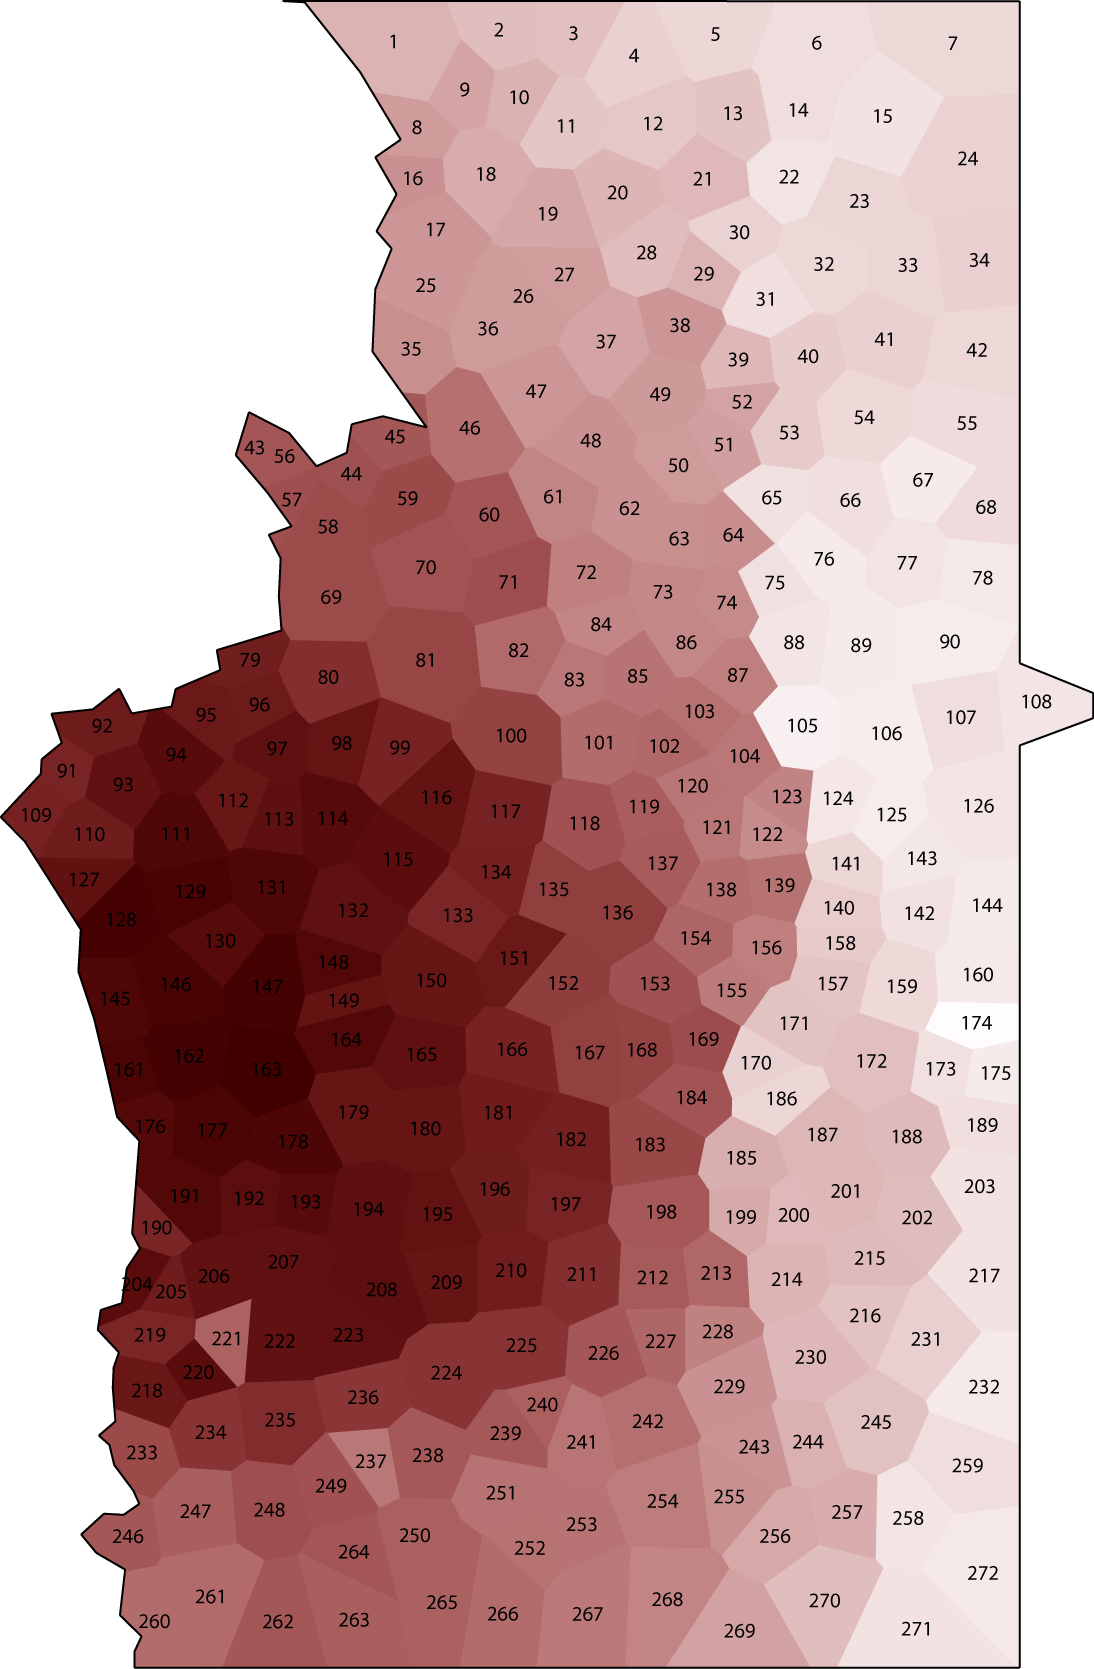
\includegraphics[width=0.3\textwidth]{illustrations/pickl_fig2}
\caption{Factor 1 (15.68~\%).}
\label{fig:2}
\end{figure}

\begin{table}
\begin{tabular}{llll}
\lsptoprule
& {\bfseries Variable (map)} & {\bfseries Variant} & {\bfseries Score}\\
\midrule

{\bfseries 1} & 
\textit{man} (before stress) (9.275) & \textit{m$\alpha $}/\textit{mə} &  6.226463\\

 {\bfseries 2} & 
\begin{minipage}[t]{0.3\textwidth}MHG \textit{ȥ} (germ. *\textit{t}) in \textit{herau}\textit{ß}\textit{en} (7.143)\end{minipage} & fricative, lenis &  6.112138\\
 
 {\bfseries 3} & 
\begin{minipage}[t]{0.3\textwidth}MHG \textit{ou} in \textit{au}\textit{ch} (5.118)\end{minipage} & {\itshape ao} &  6.045917\\
 
 {\bfseries 4} & 
\begin{minipage}[t]{0.3\textwidth}MHG \textit{ou} in \textit{(ein)k}\textit{au}\textit{fen} (5.124)\end{minipage} & {\itshape ao} &  5.823385\\
 
 {\bfseries 5} & 
\begin{minipage}[t]{0.3\textwidth}OHG Strong verbs, Class V (\textit{siehst}, 2\textsuperscript{nd} sg.) (6.58)\end{minipage} & \textit{s\={\i}š} (\textit{h} not realised) &  5.800744\\
 
 {\bfseries 6} & 
\begin{minipage}[t]{0.3\textwidth}MHG \textit{ë} in \textit{B}\textit{e}\textit{sen} (4.57)\end{minipage} & {\itshape \={e}ə} &  5.787916\\
 
 {\bfseries 7} & 
\begin{minipage}[t]{0.3\textwidth}MHG \textit{ou} in \textit{l}\textit{au}\textit{fen} (5.125)\end{minipage} & {\itshape ao} &  5.748020\\
 
 {\bfseries 8} & 
\begin{minipage}[t]{0.3\textwidth}MHG \textit{h} in \textit{sie}\textit{h}\textit{st} (7.201)\end{minipage} & \textit{h} not realised (long vowel) &  5.721860\\
 
 {\bfseries 9} & 
\begin{minipage}[t]{0.3\textwidth}MHG \textit{h} (germ. *\textit{h}) in \textit{ho}\textit{h}\textit{{}-} (7.193)\end{minipage} & \textit{h} not realised &  5.715720\\
 
 {\bfseries 10} & 
\begin{minipage}[t]{0.3\textwidth}MHG \textit{ou} in \textit{Au}\textit{ge(n)} (5.121)\end{minipage} & {\itshape ao} &  5.677732\\
 
 {\bfseries 11} & 
\begin{minipage}[t]{0.3\textwidth}MHG \textit{ou} in \textit{gl}\textit{au}\textit{ben}/\textit{Gl}\textit{au}\textit{be(n)} (5.119)\end{minipage} & {\itshape ao} &  5.645496\\
 
 {\bfseries 12} & 
\begin{minipage}[t]{0.3\textwidth}MHG \textit{b} in \textit{geglau}\textit{b}\textit{t} (7.14)\end{minipage} & \textit{b} (long vowel) &  5.631118\\
 
 {\bfseries 13} & 
\begin{minipage}[t]{0.3\textwidth}\textit{(voll)}\textit{er} (\textit{deine Hose ist ... Dreck}) (9.310)\end{minipage} & {\itshape ə} &  5.576183\\
 
 {\bfseries 14} & 
\begin{minipage}[t]{0.3\textwidth}MHG \textit{ch} in \textit{Fur}\textit{ch}\textit{e} (7.190)\end{minipage} & \textit{ch} not realised (long vowel) &  5.575329\\
 
 {\bfseries 15} & 
\begin{minipage}[t]{0.3\textwidth}OHG Strong verbs, class Ib (\textit{geschneit}, participle) (6.36)\end{minipage} & {\itshape gšn\=\iə̥} &  5.570381\\
 
 {\bfseries 16} & 
\begin{minipage}[t]{0.3\textwidth}OHG Strong verbs, class VI (\textit{trägst}, 2\textsuperscript{nd} sg.) (6.75)\end{minipage} & {\itshape drâeš} &  5.562552\\
 
 {\bfseries 17} & 
\begin{minipage}[t]{0.3\textwidth}MHG \textit{h} in \textit{(ich) se}\textit{h}\textit{e}, (\textit{er) sie}\textit{h}\textit{t} (7.197)\end{minipage} & \textit{h} not realised &  5.534073\\
 
 {\bfseries 18} & 
\begin{minipage}[t]{0.3\textwidth}MHG \textit{\^{ü} }(\textit{iu}) before \textit{l} in \textit{Säulen} (5.K3)\end{minipage} & \textit{ệi} (first element closed) &  5.521782\\
 
 {\bfseries 19} & 
\begin{minipage}[t]{0.3\textwidth}\textit{sagst}/\textit{sagt} (6.K23)\end{minipage} & \begin{minipage}[t]{0.3\textwidth}\textit{s\={e}(š)(d)}/\textit{sâe(š)(d)} (\textit{g} not realised)\end{minipage} &  5.508044\\
 
 {\bfseries 20} & 
\begin{minipage}[t]{0.3\textwidth}MHG \textit{k} in \textit{On}\textit{k}\textit{el} (7.93c)\end{minipage} & unaspirated, fortis &  5.423593\\
 
\lspbottomrule
\end{tabular}
\caption{Top 20 features of Factor 1. MHG: Middle High German. OHG: Old High German.}
\label{tab:1}
\end{table}

%Figures~3–10 %%% fix reference or numbering (see below)
Figures~3–10 show the geographic distributions of all the other dominant factors (Factors 2–7, 10–11), i.e. of all the factors that are strongest at one location at least. The explained variances are given in brackets. Divergent colours in the individual maps represent negative loadings. 

%%%
%%% using subcaption package (don't forget to include)
%%%
%%% fix subfigure numbering OR reference text to match them up
%%%
\begin{figure}
\centering
\begin{subfigure}[t]{0.3\textwidth}
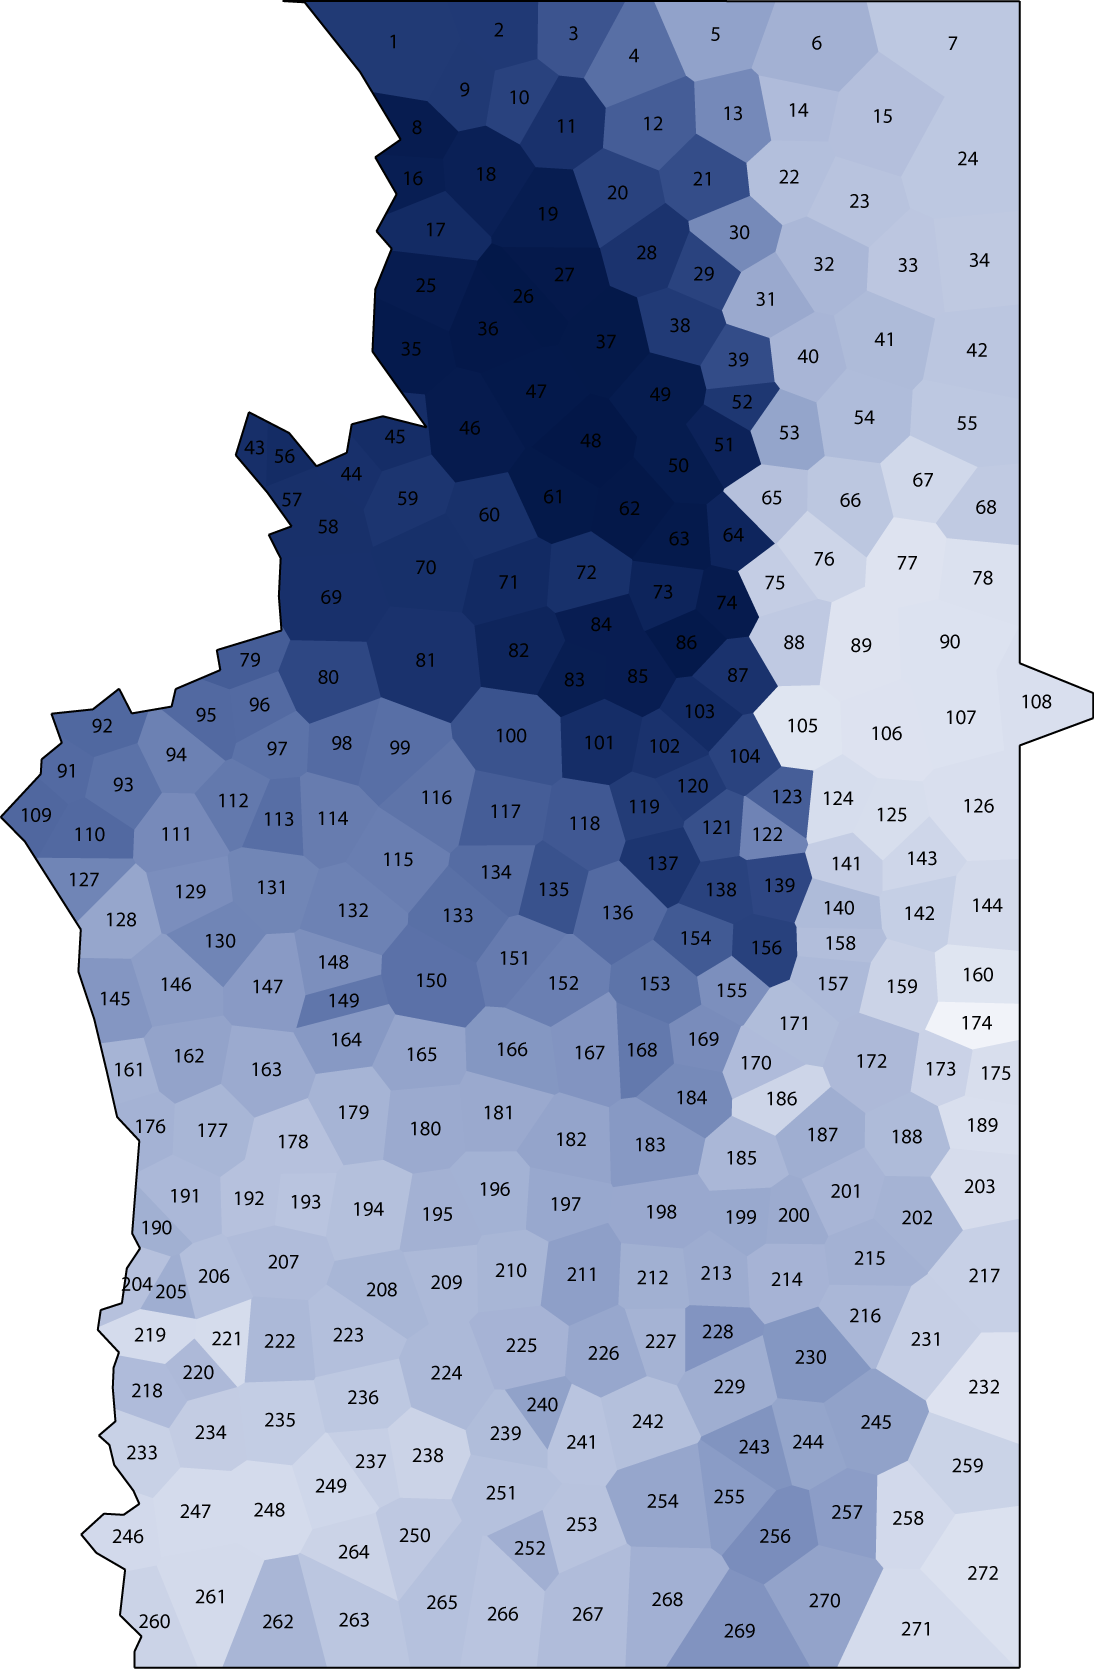
\includegraphics[width=\textwidth]{illustrations/pickl_fig3}
\caption{\figref{fig:3}: Factor 2 (14.04~\%).}
\label{fig:3}
\end{subfigure}   
~
\begin{subfigure}[t]{0.3\textwidth}
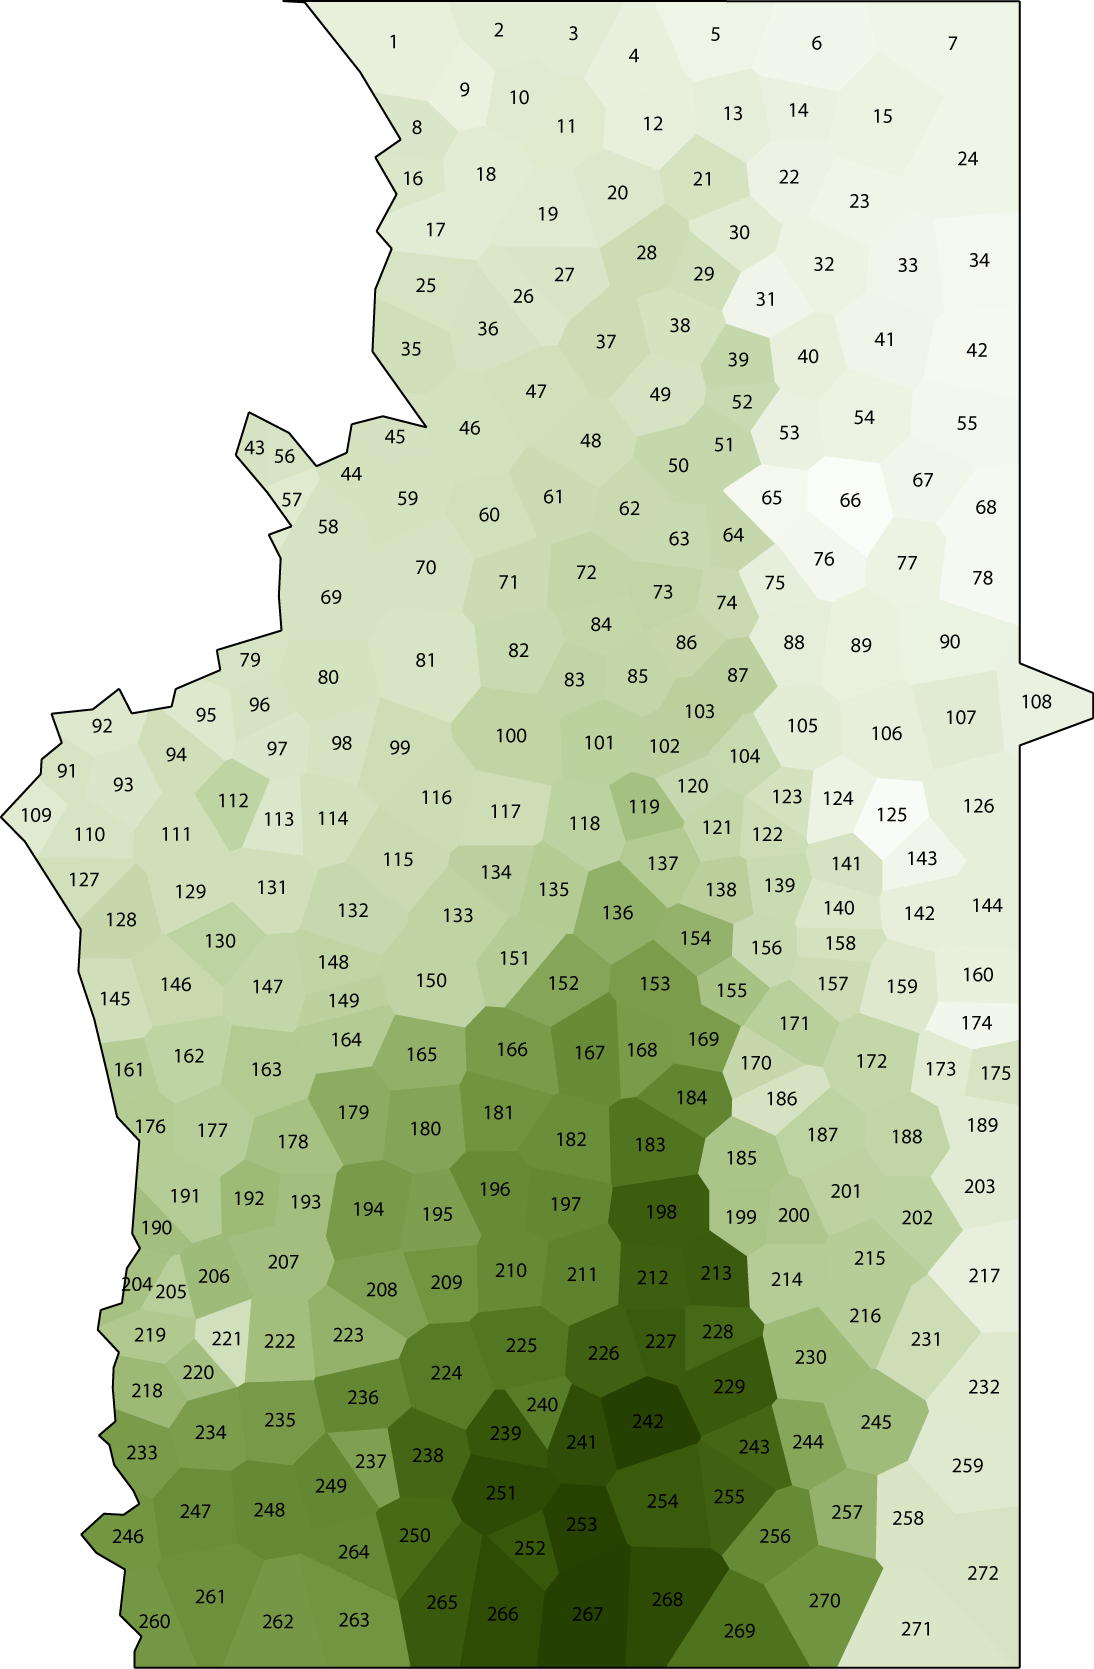
\includegraphics[width=\textwidth]{illustrations/pickl_fig4}
\caption{\figref{fig:4}: Factor 3 (8.98~\%).}
\label{fig:4}
\end{subfigure}  
~
\begin{subfigure}[t]{0.3\textwidth}
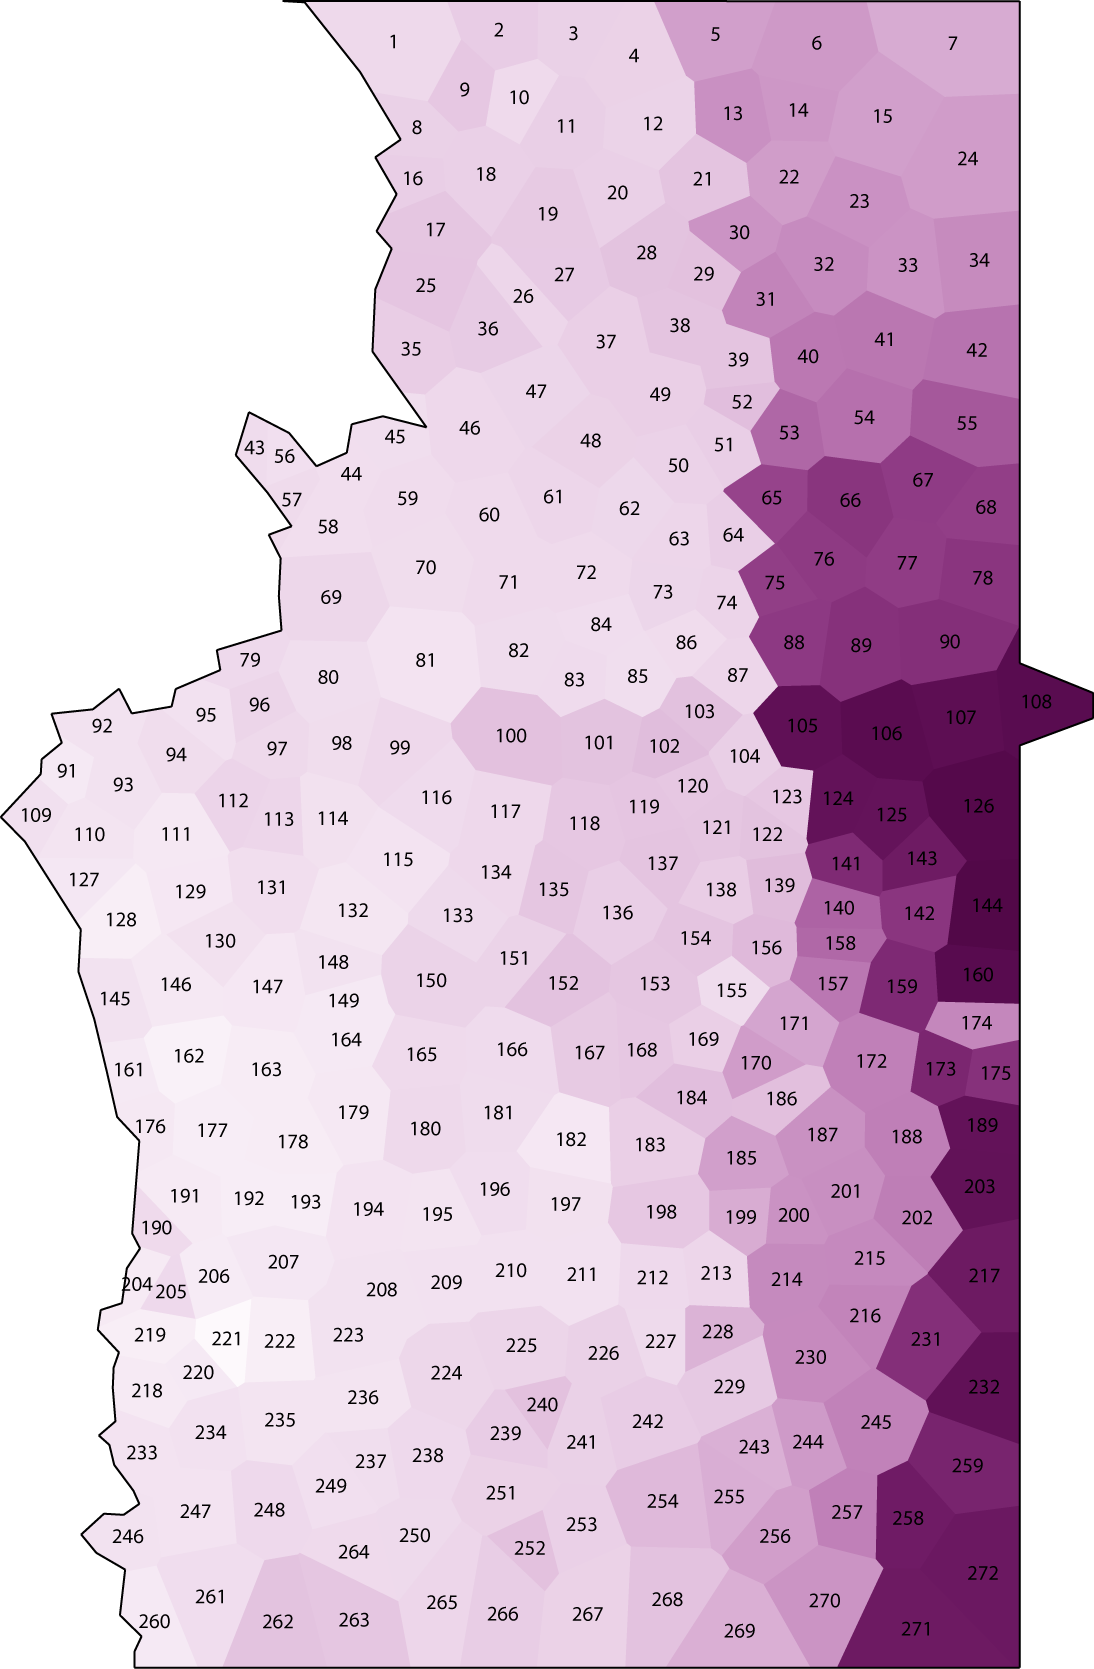
\includegraphics[width=\textwidth]{illustrations/pickl_fig5}
\caption{\figref{fig:5}: Factor 4 (5.74~\%).}
\label{fig:5}
\end{subfigure}

\vskip11pt

\begin{subfigure}[t]{0.3\textwidth}
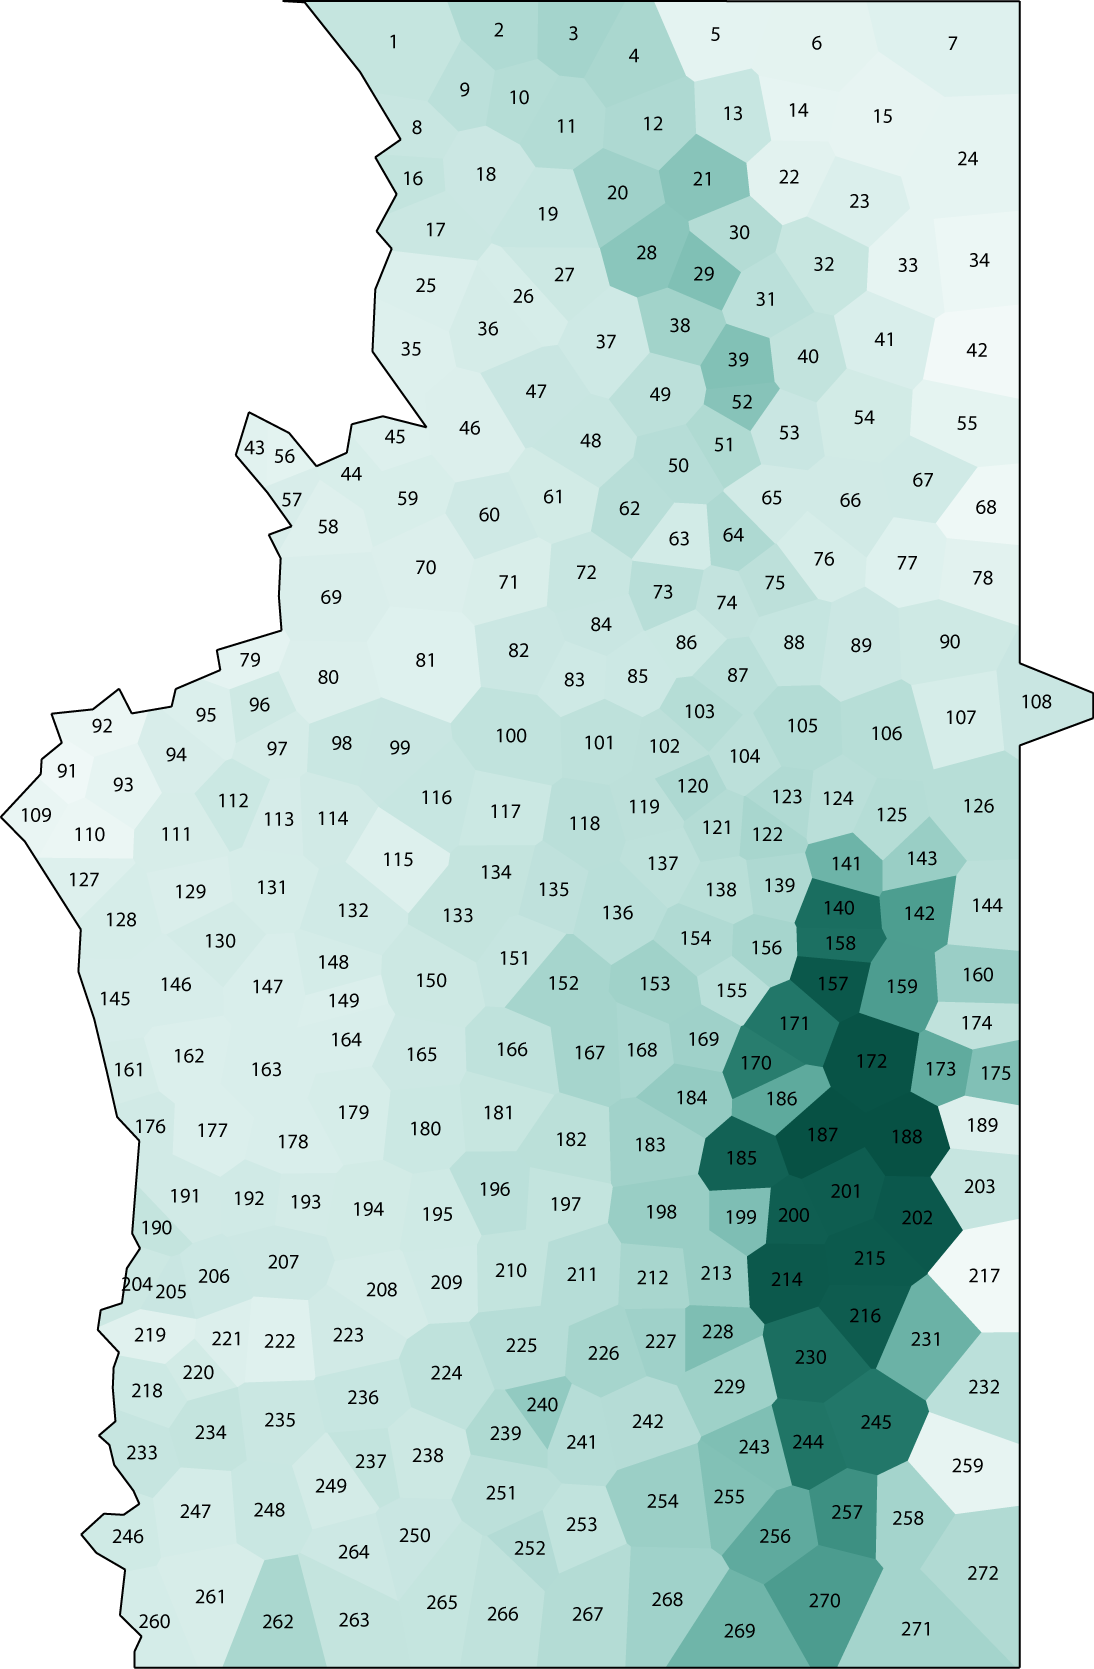
\includegraphics[width=\textwidth]{illustrations/pickl_fig6}
\caption{\figref{fig:6}: Factor 5 (4.68~\%).}
\label{fig:6}
\end{subfigure}   
~
\begin{subfigure}[t]{0.3\textwidth}
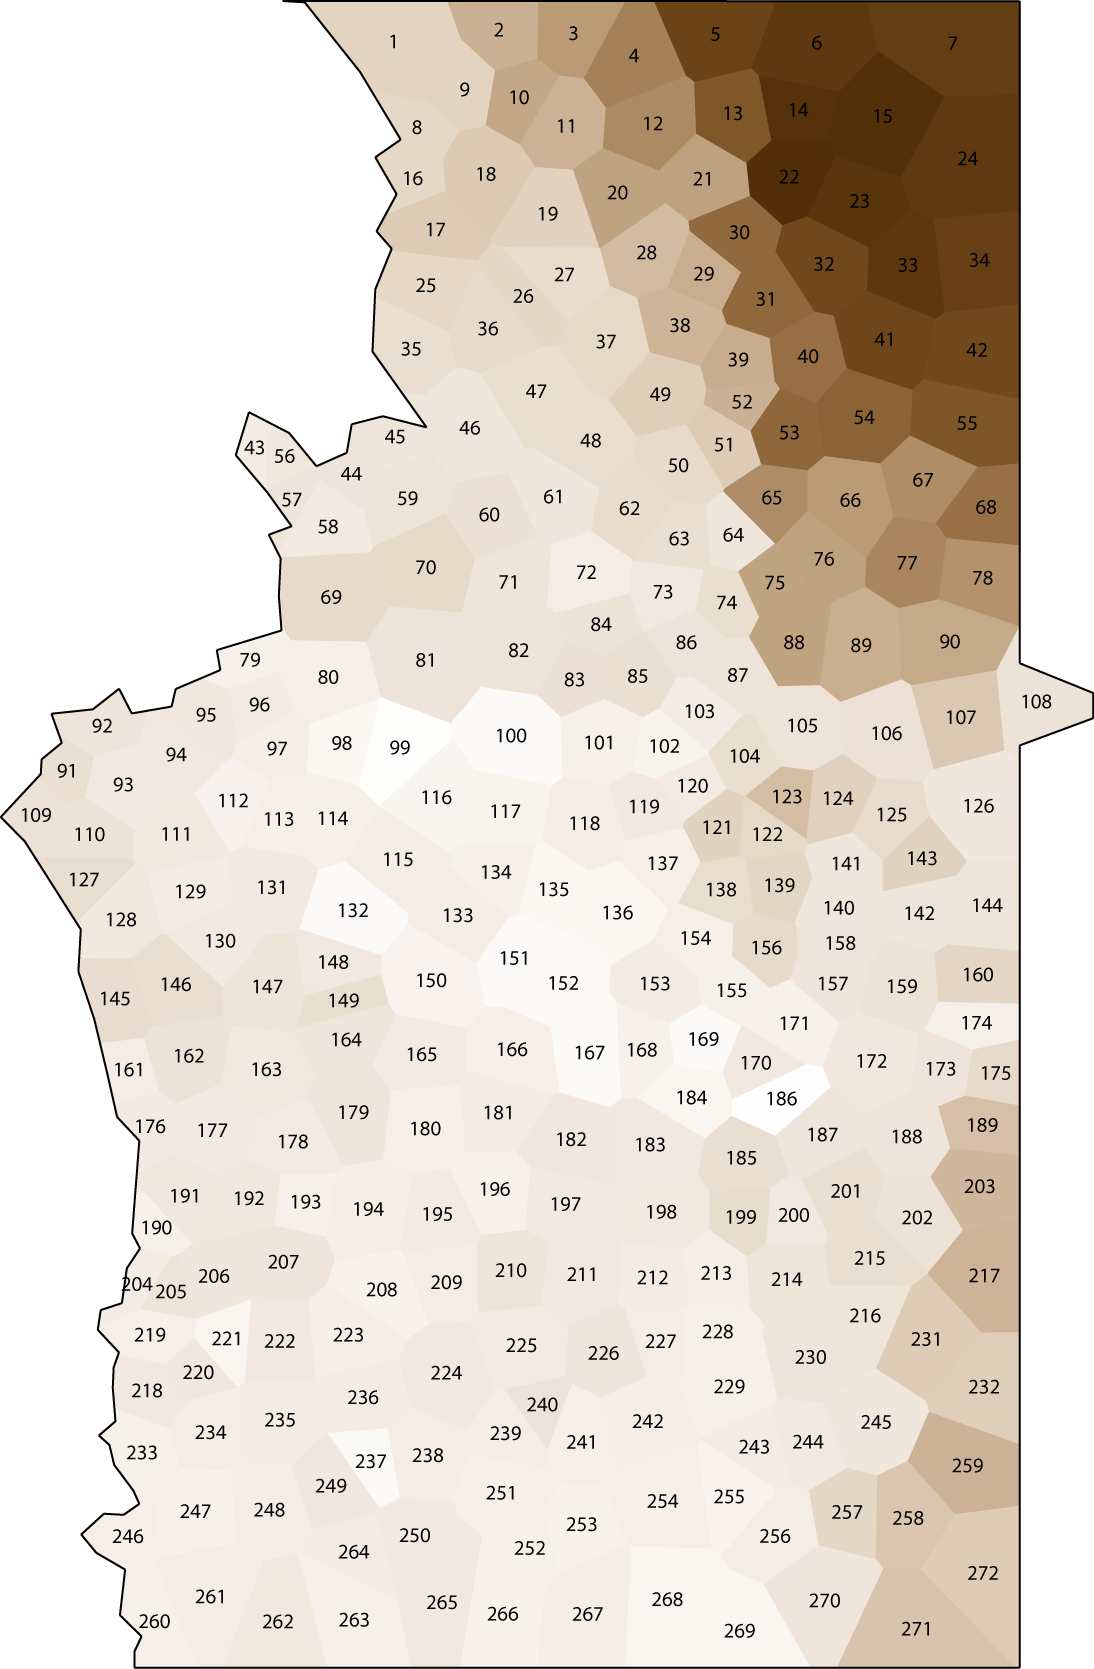
\includegraphics[width=\textwidth]{illustrations/pickl_fig7}
\caption{\figref{fig:7}: Factor 6 (3.88~\%).}
\label{fig:7}
\end{subfigure}  
~
\begin{subfigure}[t]{0.3\textwidth}
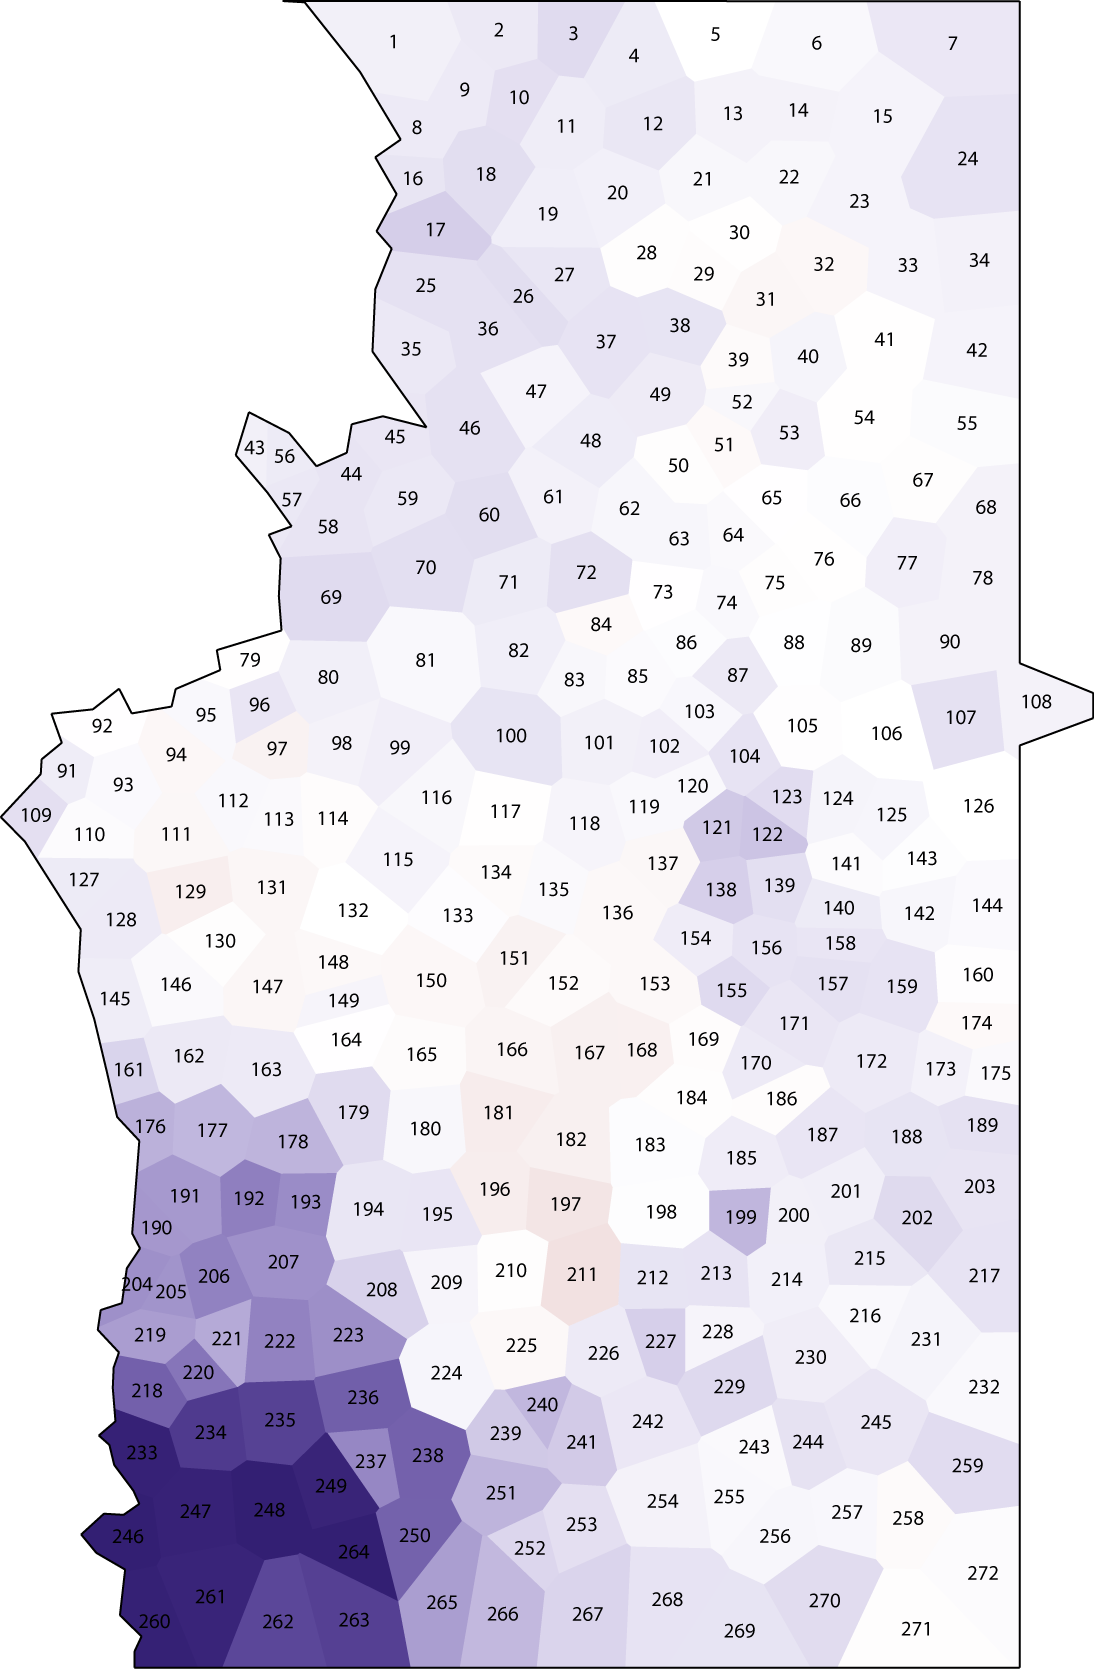
\includegraphics[width=\textwidth]{illustrations/pickl_fig8}
\caption{\figref{fig:8}: Factor 7 (1.91~\%).}
\label{fig:8}
\end{subfigure}
\end{figure}

\begin{figure}
\begin{subfigure}[t]{0.3\textwidth}
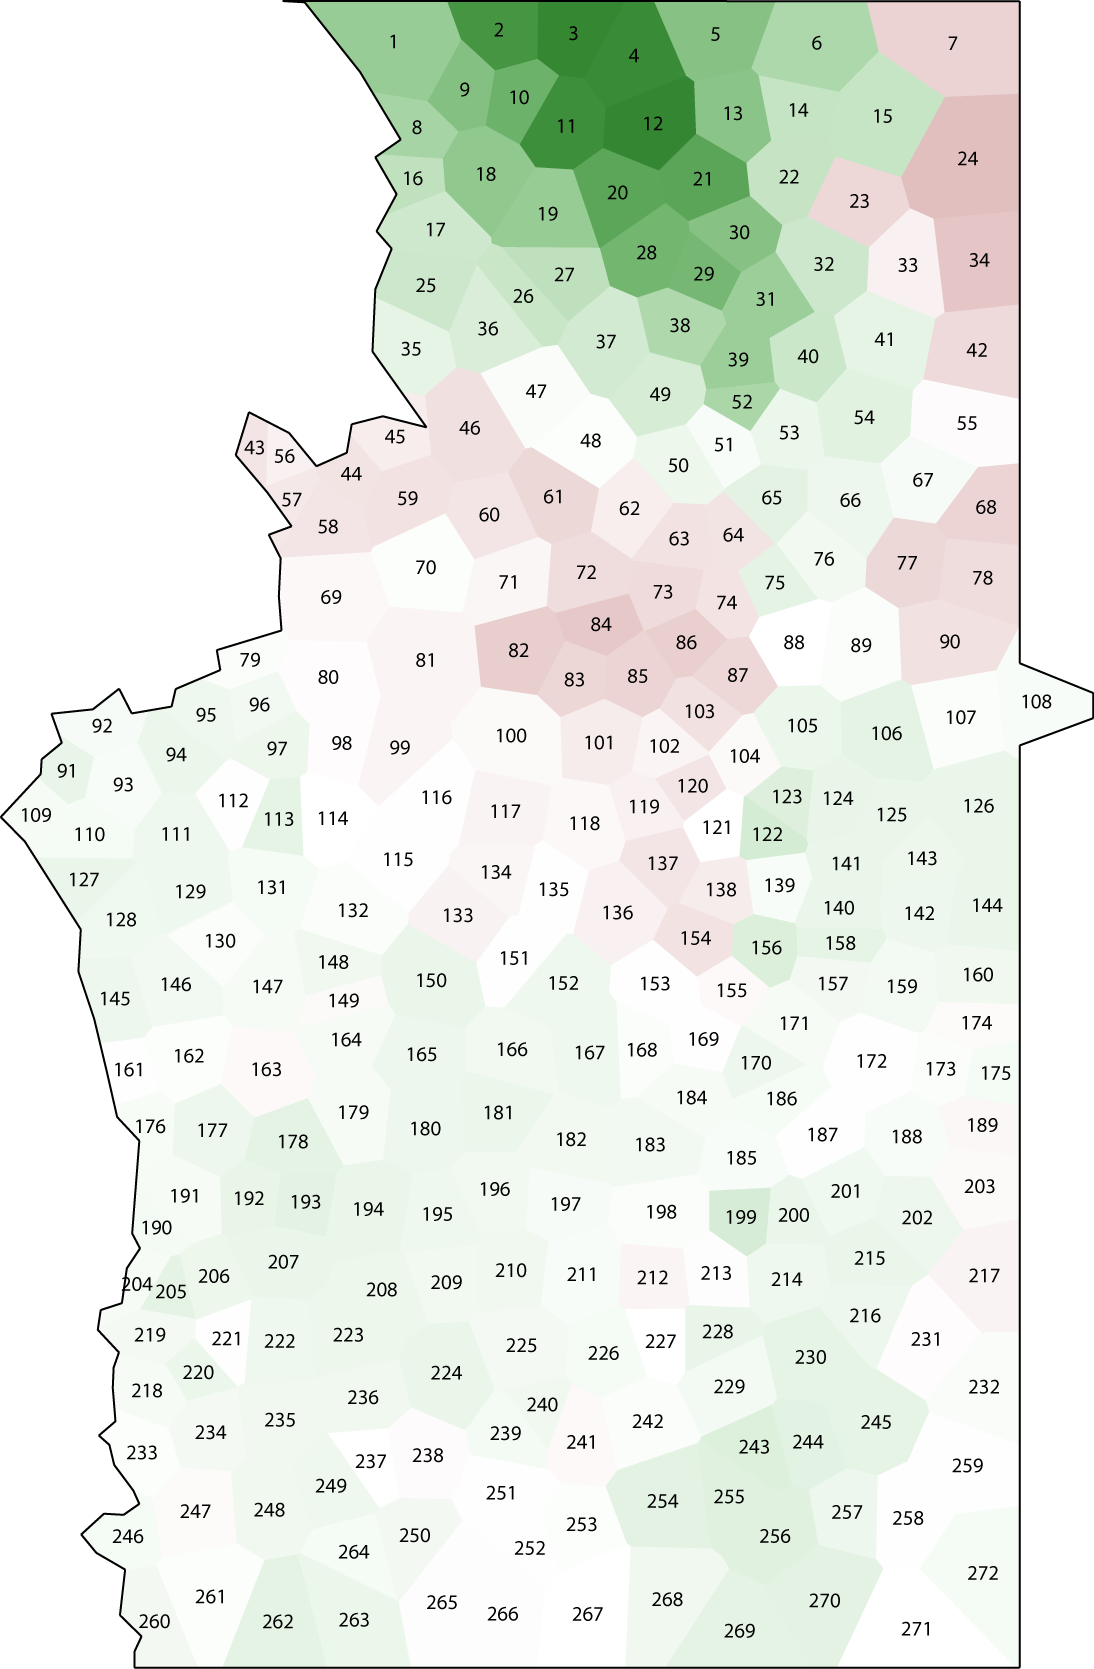
\includegraphics[width=\textwidth]{illustrations/pickl_fig9}
\caption{\figref{fig:9}: Factor 10 (1.02~\%).}
\label{fig:9}
\end{subfigure}   
~
\begin{subfigure}[t]{0.3\textwidth}
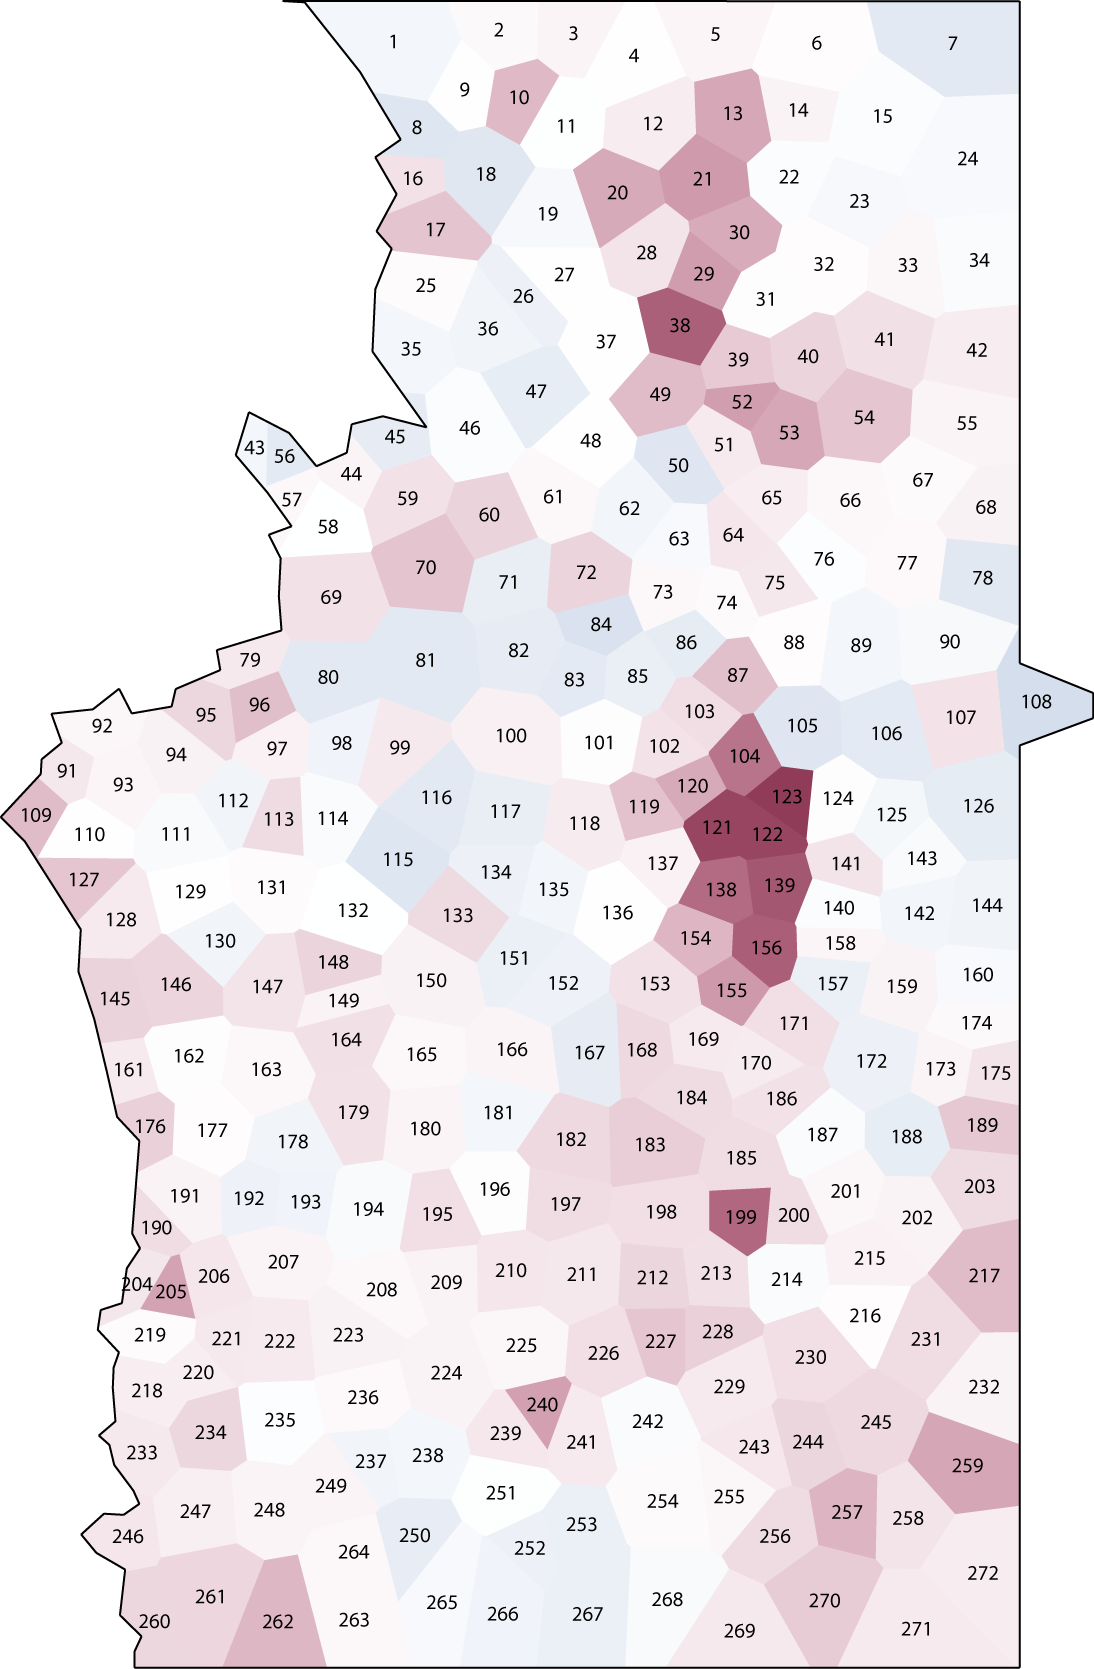
\includegraphics[width=\textwidth]{illustrations/pickl_fig10}
\caption{\figref{fig:10}: Factor 11 (0.85~\%).}
\label{fig:10}
\end{subfigure}  
~
\begin{subfigure}[t]{0.3\textwidth}
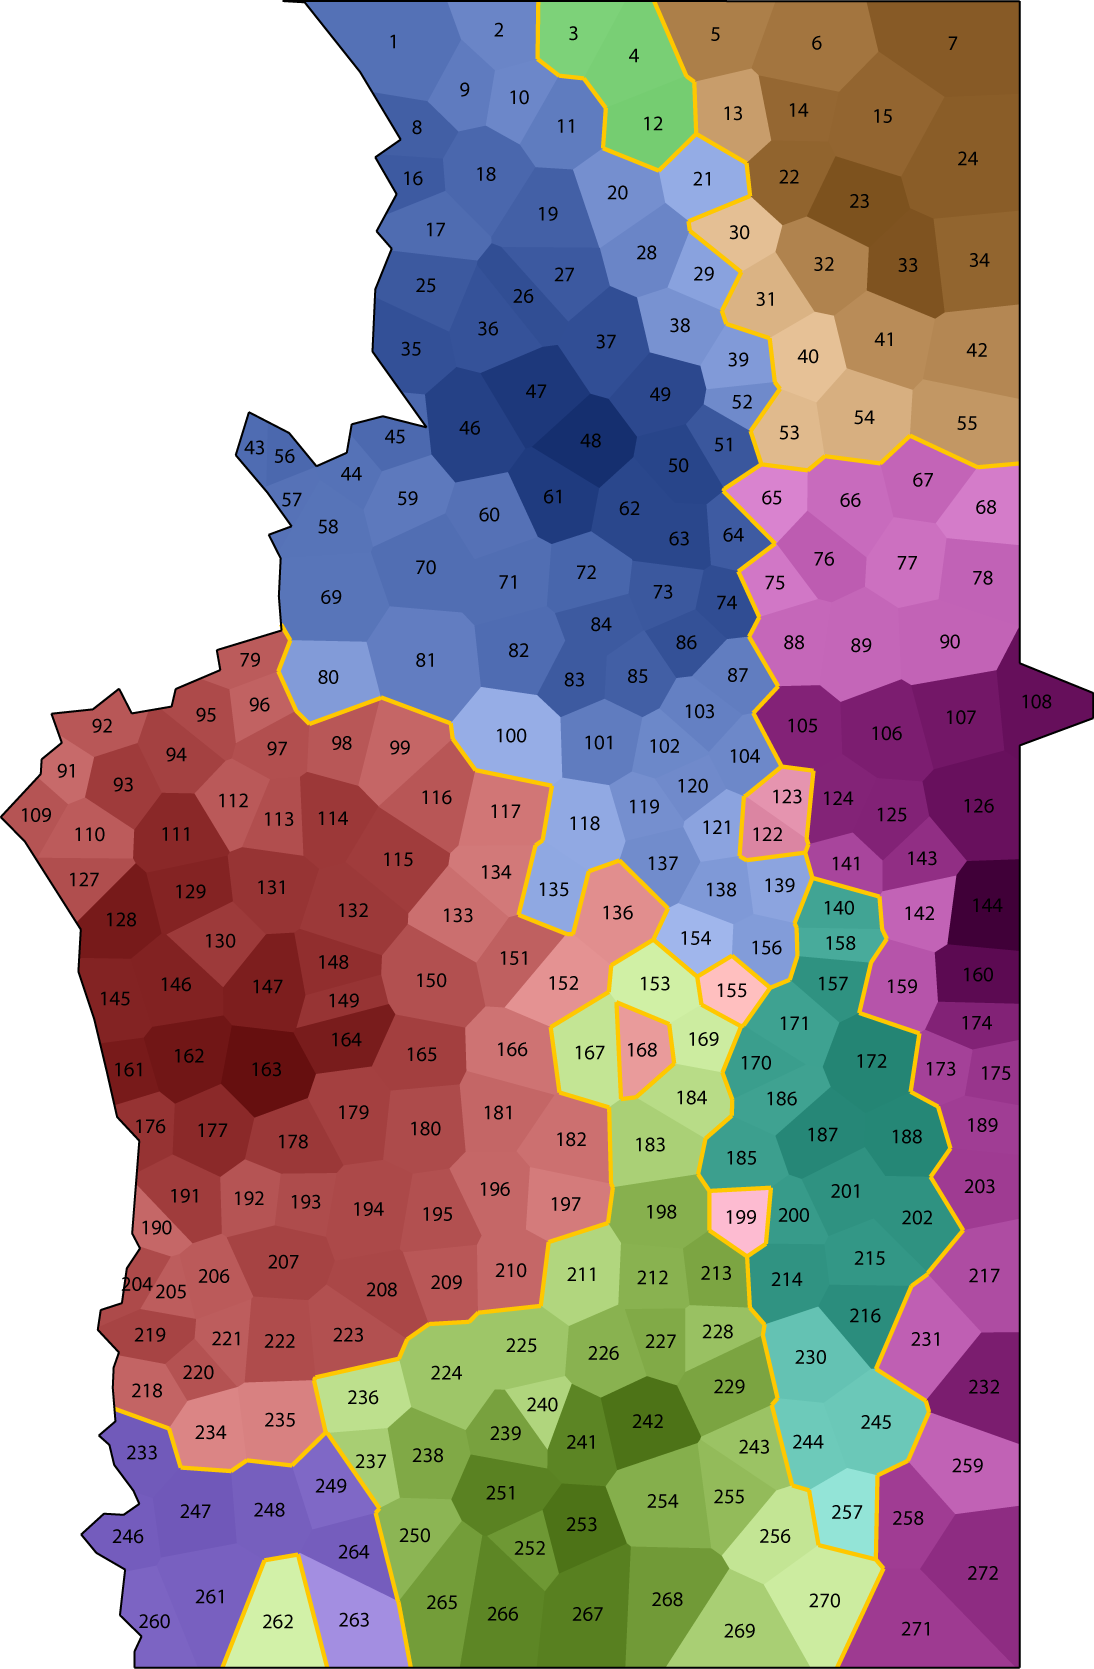
\includegraphics[width=\textwidth]{illustrations/pickl_fig11}
\caption{\figref{fig:11}: Combined factor map.}
\label{fig:11}
\end{subfigure}
\end{figure}

Most of these factors can be associated with traditional dialect areas: Factor 2 with North East Swabian, Factor 3 with East Algovian, Factor 4 with Central Bavarian, Factor 5 with Lechrainian, Factor 6 with Northern Bavarian, Factor 7 with West Algovian, Factor 10 with East Franconian. Factor 11 appears to capture variants that are characteristic for towns and cities: The agglomeration around location 122 is the metropolitan area of Augsburg, and most of the other locations with high loadings are larger towns: Landsberg am Lech (199), Memmingen (205), Kaufbeuren (240), Weilheim (Oberbayern) (259), Neu-Ulm (109), Günzburg (96), Dillingen (70), Kaisheim (38), Rain am Lech (53), Donauwörth (49), Nördlingen (17), Oettingen (10), Monheim (30) with its boroghs Itzing (29) and Weilheim (21), Wemding (20), Möhren (13) (borough of Treuchtlingen). The correlation between Factor 11’s loadings and the populations\footnote{Figures for 1971 are taken from: \citet{bayerisches_statistisches_landesamt_einwohnerzahlen_1972}.} of all 272 locations is 0.45, which corresponds to an explained variance of \textit{R}\textsuperscript{2}~=~20~\%; the logarithmic relation is somewhat stronger (\textit{R}\textsuperscript{2}~=~28~\%). Factor 11, therefore, can be interpreted as a geographically discontinuous urban variety; it captures variants that are used predominantly and typically in larger towns and cities. Table~2 lists the top 20 features for this type. The preservation of vowel shortness (2, 3, 4, 5, 6, 8, 12, 15, 16, 17, 18, 20) seems to be especially characteristic of this factor. It does come as a surprise that almost all of the variants are identical with the respective standard variants. The lenition of plosives and fricatives (1, 10, 19, 20) seems to be an exception (except for 10, where lenition occurs also in the standard), which would qualify it as a unique feature of regional urbanity that is distinct from the standard.

\begin{table}
\begin{tabular}{llll} 
\lsptoprule
& {\bfseries Variable (map)} & {\bfseries Variant} &  {\bfseries Score}\\
\midrule

 {\bfseries 1} & 
 \begin{minipage}[t]{0.3\textwidth}MHG \textit{pf} after \textit{m}, word-final (\textit{Dam}\textit{pf}, \textit{Strum}\textit{pf}) (7.215)\end{minipage} & lenis affricate &  8.066857\\
 
 {\bfseries 2} & 
 \begin{minipage}[t]{0.3\textwidth}\textit{i} before \textit{ch} (\textit{St}\textit{i}\textit{ch(e)}) (sg./pl.) (3.2)\end{minipage} & short vowel &  7.848610\\
 
 {\bfseries 3} & 
 \begin{minipage}[t]{0.3\textwidth}Vowel quantity in \textit{St}\textit{i}\textit{ch(e)} (sg./pl.) (9.30)\end{minipage} & short vowel in singular and plural &  7.548978\\
 
 {\bfseries 4} & 
 \begin{minipage}[t]{0.3\textwidth}\textit{o} before fortis fricative (\textit{Fr}\textit{o}\textit{sch}) (3.8)\end{minipage} & short vowel &  7.436807\\
 
 {\bfseries 5} & 
 \begin{minipage}[t]{0.3\textwidth}Vowel quantity in \textit{D}\textit{a}\textit{rm }(3.66)\end{minipage} & short vowel &  7.253476\\
 
 {\bfseries 6} & 
 \begin{minipage}[t]{0.3\textwidth}MHG \textit{i}/\textit{u} in \textit{Z}\textit{i}\textit{nken }(4.47)\end{minipage} & short open \textit{i} (monophthong) &  7.102994\\
 
 {\bfseries 7} & 
 \begin{minipage}[t]{0.3\textwidth}MHG \textit{u}/\textit{o} in \textit{d}\textit{o}\textit{nnern} (4.49)\end{minipage} & neutral/closed \textit{o} &  7.009078\\
 
 {\bfseries 8} & 
 \begin{minipage}[t]{0.3\textwidth}Vowel quantity in \textit{F}\textit{i}\textit{rst }(3.42)\end{minipage} & short vowel &  6.999477\\
 
 {\bfseries 9} & 
 \begin{minipage}[t]{0.3\textwidth}Gender of \textit{Teller} (9.165)\end{minipage} & masculine &  6.919323\\
 
 {\bfseries 10} & 
 \begin{minipage}[t]{0.3\textwidth}MHG \textit{t} after nasal, word-final (\textit{tausen}\textit{d}) (7.K68c)\end{minipage} & lenis plosive &  6.914453\\
 
 {\bfseries 11} & 
 \begin{minipage}[t]{0.3\textwidth}\textit{im (Bett)} (9.373)\end{minipage} & {\itshape \k{i}m} &  6.901412\\
 
 {\bfseries 12} & 
 \begin{minipage}[t]{0.3\textwidth}\textit{a}/\textit{o} before \textit{ch} (\textit{B}\textit{a}\textit{ch}/\textit{D}\textit{a}\textit{ch}/\textit{L}\textit{o}\textit{ch}) (3.1)\end{minipage} & short vowel &  6.759506\\
 
 {\bfseries 13} & 
 \begin{minipage}[t]{0.3\textwidth}MHG \textit{â} in \textit{Sal}\textit{a}\textit{t} (5.55)\end{minipage} & neutral \textit{\=a} &  6.635629\\
 
 {\bfseries 14} & 
 \begin{minipage}[t]{0.3\textwidth}\textit{{}-ig} in \textit{Kön}\textit{ig} (9.26)\end{minipage} & {\itshape {}-ig} &  6.581771\\
 
 {\bfseries 15} & 
 \begin{minipage}[t]{0.3\textwidth}MHG \textit{o} before \textit{pf} in \textit{K}\textit{o}\textit{pf} (4.100a)\end{minipage} & short closed \textit{o} (monophthong) &  6.542050\\
 
 {\bfseries 16} & 
 \begin{minipage}[t]{0.3\textwidth}Vowel quantity in \textit{St}\textit{a}\textit{ll }(3.26)\end{minipage} & short vowel &  6.491926\\
 
 {\bfseries 17} & 
 \begin{minipage}[t]{0.3\textwidth}MHG \textit{o} before \textit{pf} in \textit{Z}\textit{o}\textit{pf} (4.100c)\end{minipage} & short closed \textit{o} (monophthong) &  6.490776\\
 
 {\bfseries 18} & 
 \begin{minipage}[t]{0.3\textwidth}unorganic \textit{r} in \textit{waten} and \textit{Schatten} (7.254)\end{minipage} & no \textit{r}, short vowel &  6.323896\\
 
 {\bfseries 19} & 
 \begin{minipage}[t]{0.3\textwidth}MHG \textit{t} in \textit{Feier}\textit{t}\textit{ag} (7.74)\end{minipage} & lenis plosive (\textit{r} realised) &  6.303051\\
 
 {\bfseries 20} & 
 \begin{minipage}[t]{0.3\textwidth}MHG \textit{pf} in \textit{Ko}\textit{pf}\textit{ }(7.216)\end{minipage} & lenis affricate, short vowel &  6.246637\\
 
\lspbottomrule
\end{tabular}
\caption{Top 20 features of Factor 11.}
\label{tab:2}
\end{table}

In Figure~11, all dominant factors are combined into one map, with each location assigned to the locally dominant factor. Consequently, only information about the locally dominant factors is depicted, which means that only the surface of the dialectal landscape is visible. The resulting division into areas is in principle comparable to classifications obtained using cluster analysis or similar methods. A distinction of the present map lies in the colour shades of the individual locations, which represent the different degrees of dialect area membership. Another benefit of these results is that there is variation ‘below’ the threshold of dominance, which is not visible in Figure~11 but latently present. This variation belongs firstly to the locally non-dominant parts of the globally dominant factors: each factor has loadings other than zero outside of its dominance area, but these proportions are hidden. However, they can be viewed by regarding one factor at a time (Figures~2–10).
%(Figures~2–10). 

There are also factors that are dominant nowhere in the area under investigation. They do not show up in Figure~11 at all, but again, they are latently present and can be viewed individually (Figures~12–18). Summarising small fractions of the data, they contribute to a more complete picture of overall variation and the dialectal landscape, even though they represent non-dominant dialect types, dialect areas without a core area. Many of the factors can be interpreted in a meaningful way. Several of the factors shown in Figures~12–18 seem to be related to (former) market towns: their central areas (and in some cases also their counter-centres with negative values, in red) coincide with the respective market towns’ catchment areas (as documented in Volume~1 of the SBS). For Factor 12, the blue centre correlates with the catchment area of (Neu-)Ulm (109), the red centre with the catchment area of Mindelheim (195); for Factor 13, the blue centre correlates with the catchment area of Lauingen; for Factor 14, the blue centre correlates with the catchment area of Nördlingen (17), the red centre with that of Wertingen (72); for Factor 15, the blue centre correlates with the catchment area of Jettingen, the red centre with the catchment area of Memmingen (205), for Factor 16, the blue centre correlates with the catchment areas of Schongau and Weilheim (Oberbayern) (259), the red centre with the catchment area of Mering (158).\footnote{For similar findings for lexically-based factors and a more in-depth discussion, see \citet[170--196]{pickl_probabilistische_2013}; \citet{buhler_dialektraume_2014}.} These effects are relatively weak – the factors have between 0.51~\% and 0.85~\% of explained variance, which is, however, still the equivalent of 76 to 126 variants and their distributions, and they are clearly associated with their respective counterparts. Hence it is justified to speak of non-dominant dialect types that are constituted by features characteristic of these towns’ surrounding areas. With these findings, a level of detail and depth is reached that goes beyond what has been attainable with previous methods of dialect classification.



%%%
%%% using subcaption package (don't forget to include)
%%%
%%% fix subfigure numbering OR reference text to match them up
%%%
\begin{figure}
\centering
\begin{subfigure}[t]{0.3\textwidth}
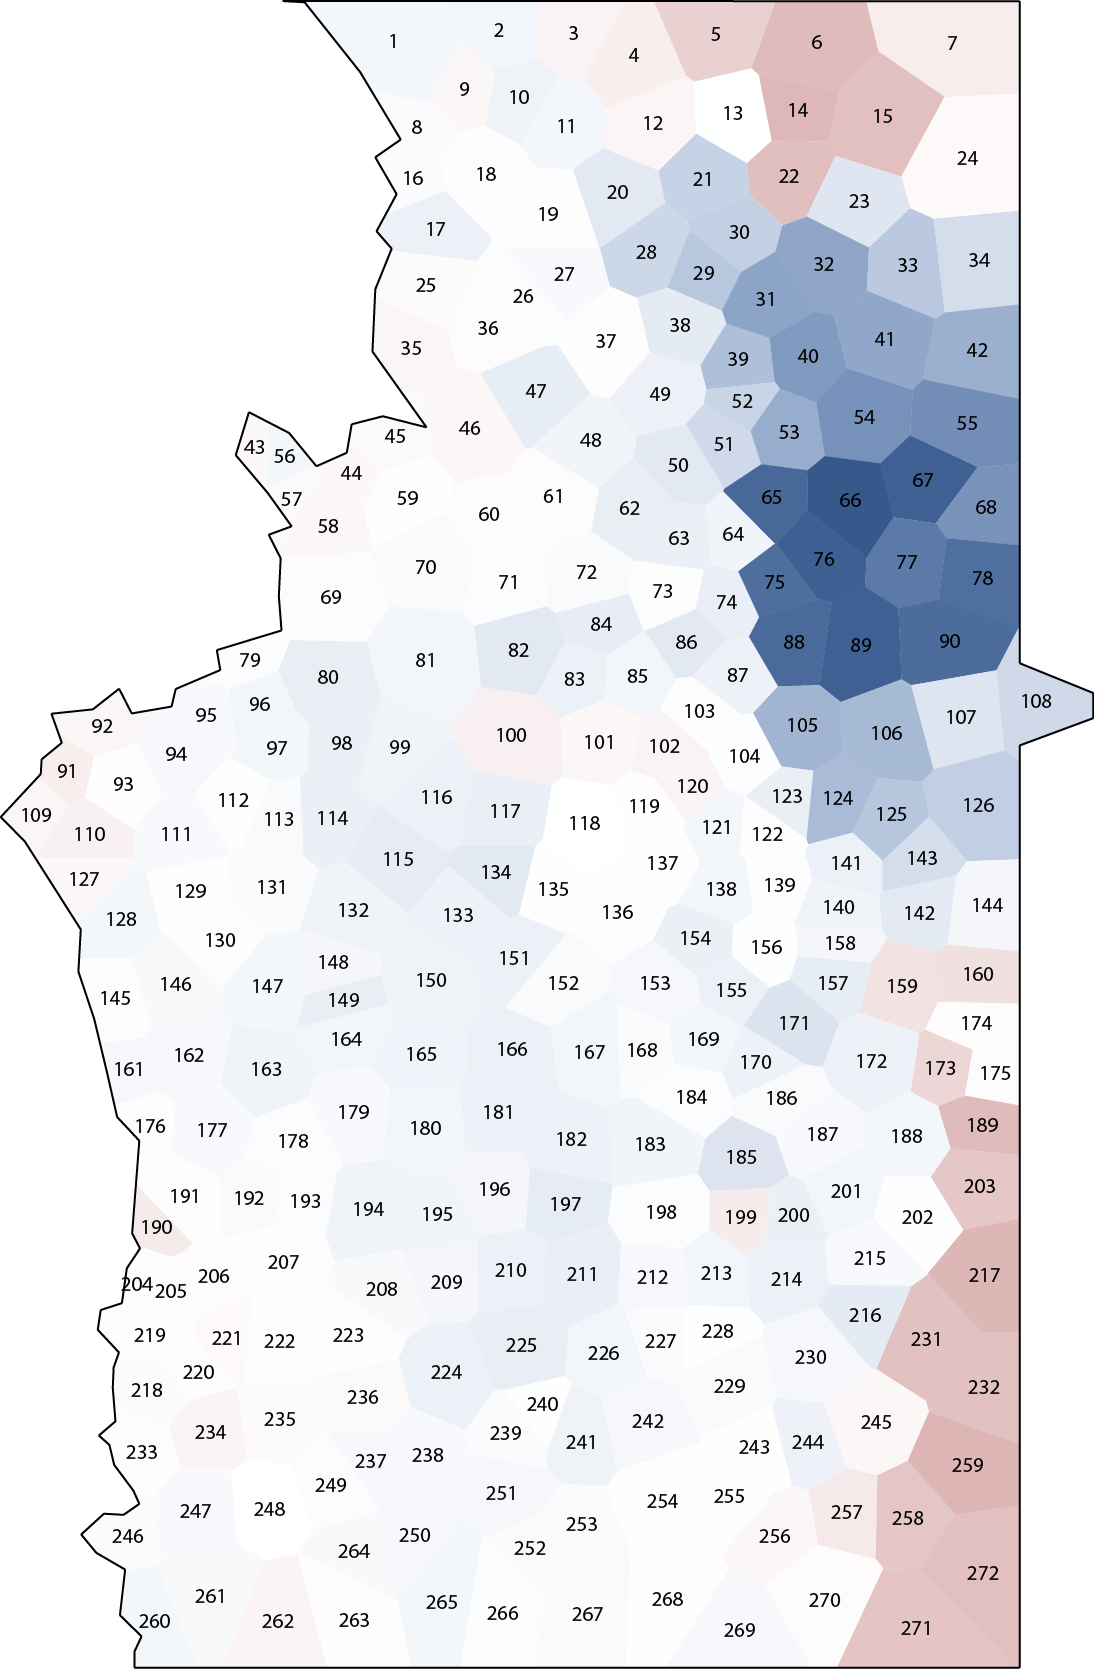
\includegraphics[width=\textwidth]{illustrations/pickl_fig12}
\caption{\figref{fig:12}: Factor 8 (1.11~\%).}
\label{fig:12}
\end{subfigure}   
~
\begin{subfigure}[t]{0.3\textwidth}
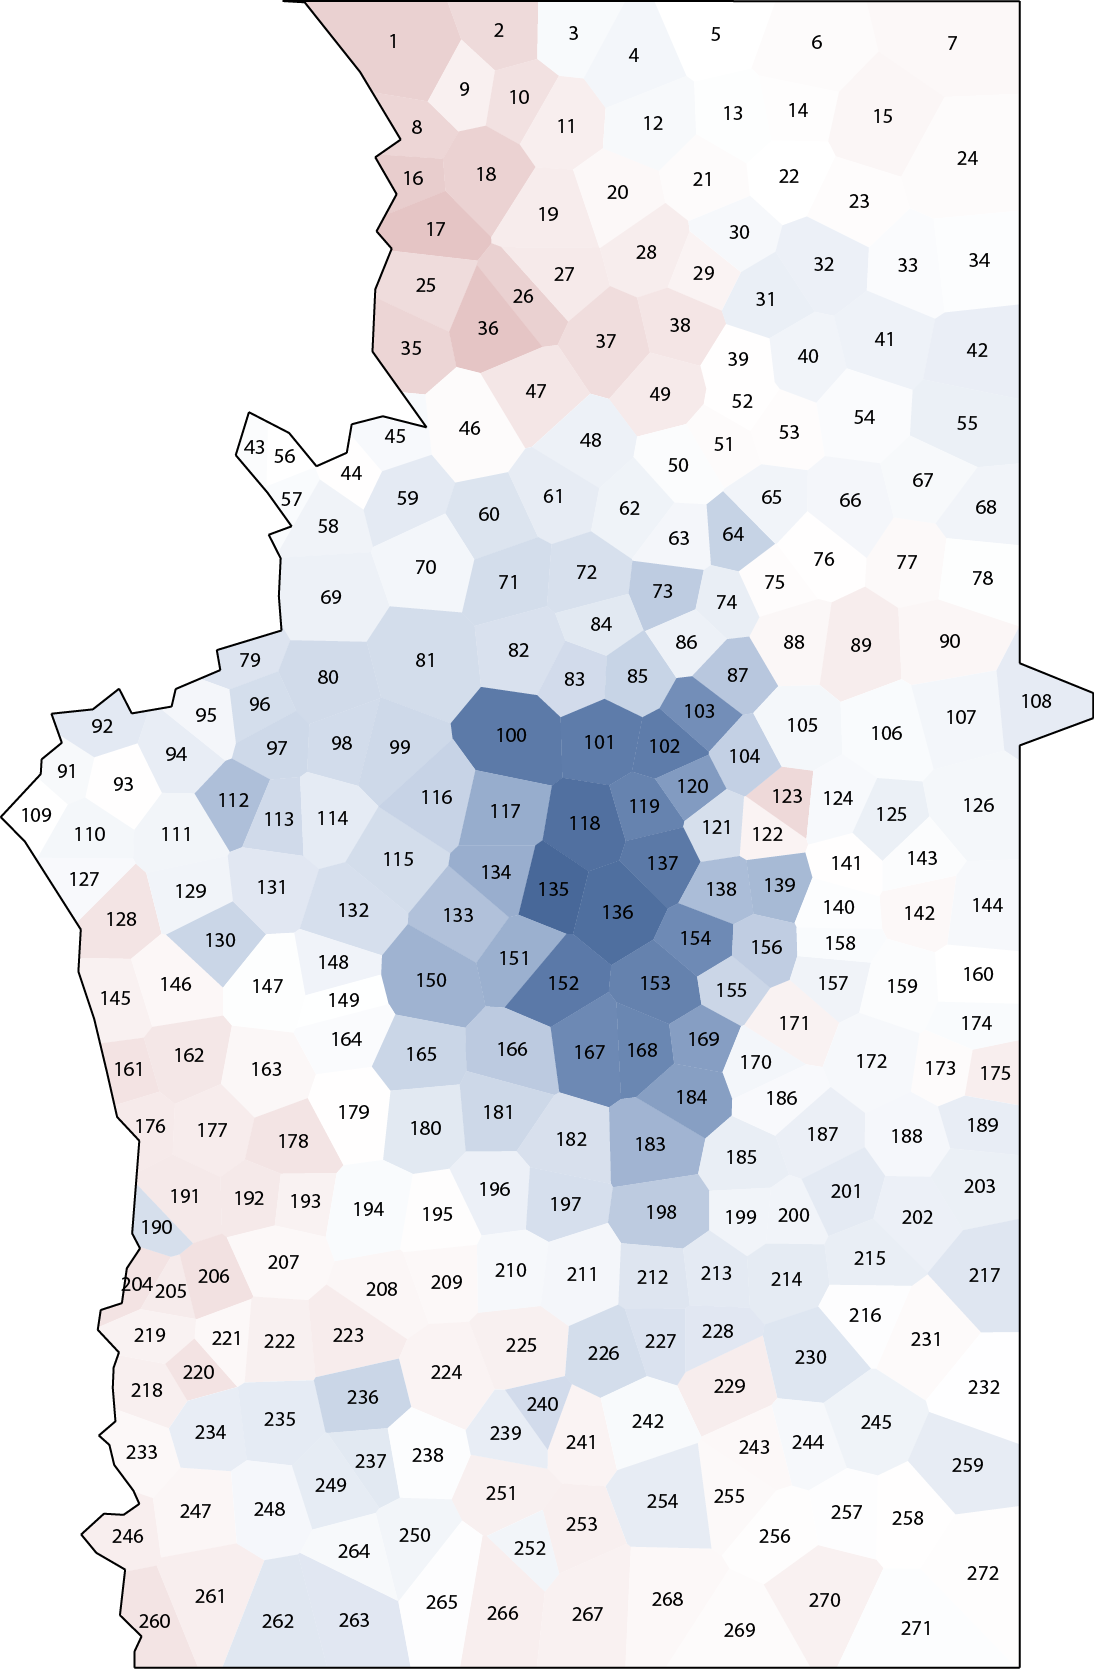
\includegraphics[width=\textwidth]{illustrations/pickl_fig13}
\caption{\figref{fig:13}: Factor 9 (1.03~\%).}
\label{fig:13}
\end{subfigure}  
~
\begin{subfigure}[t]{0.3\textwidth}
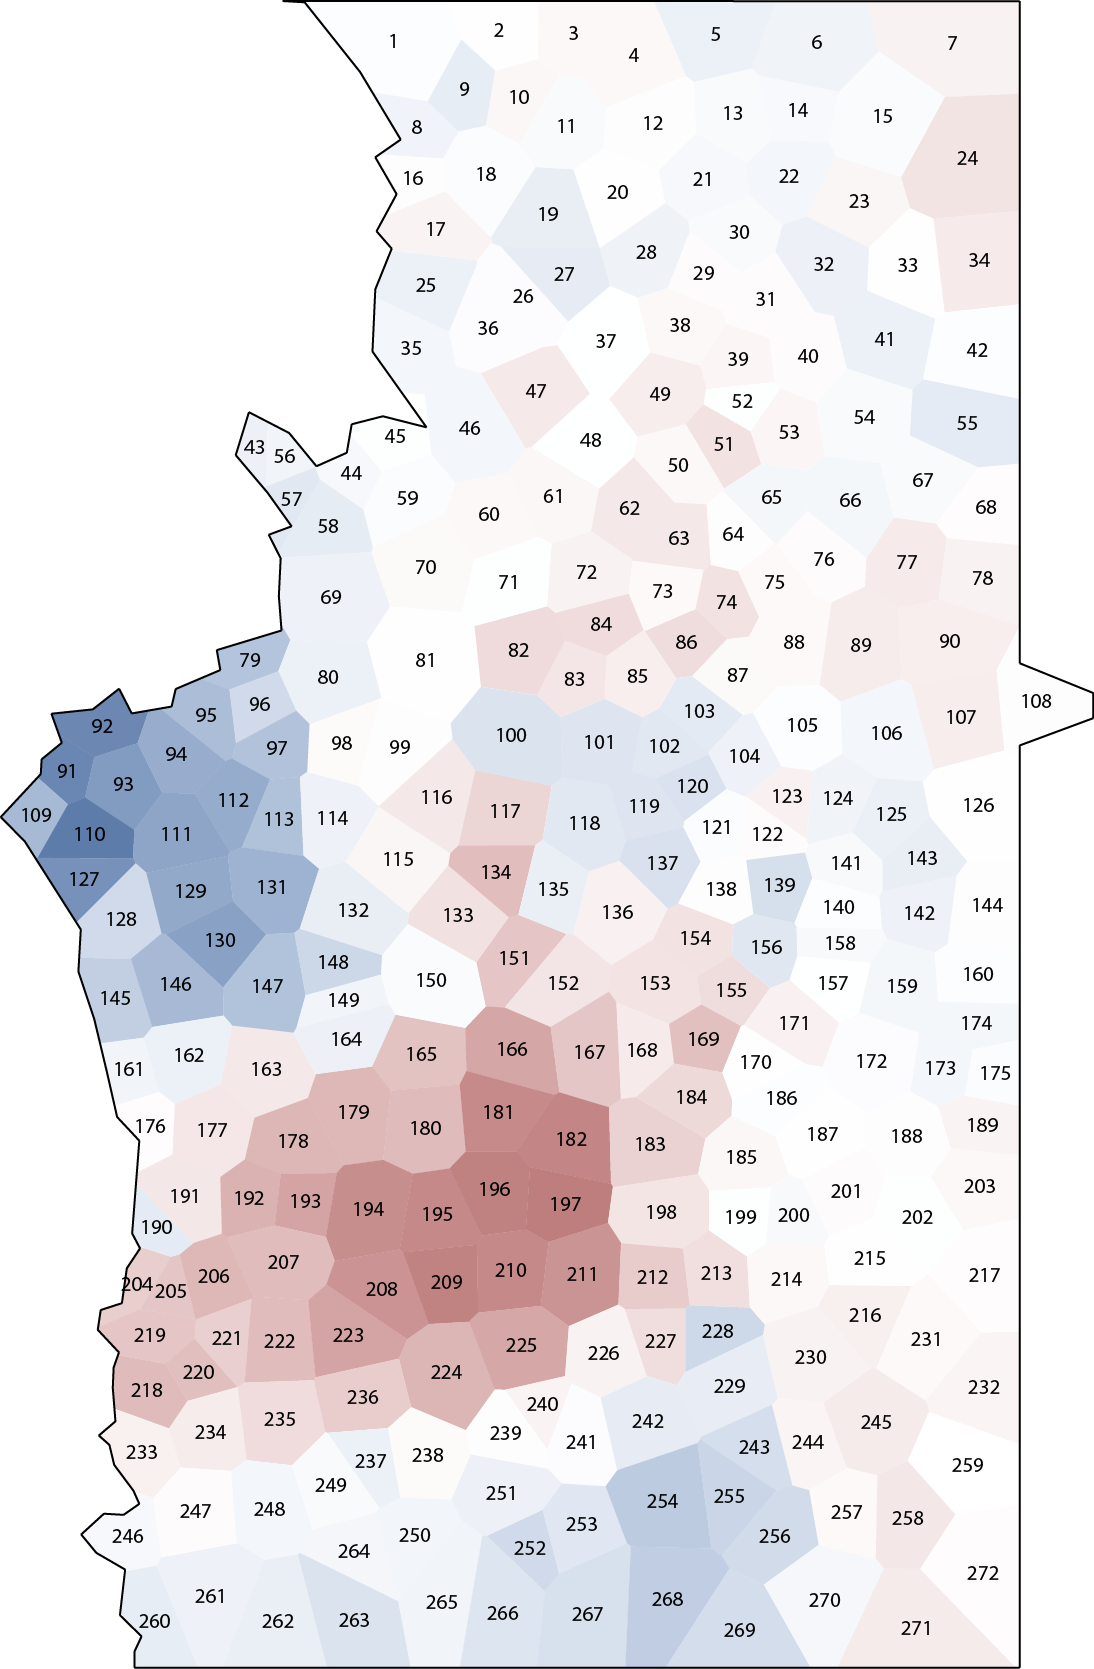
\includegraphics[width=\textwidth]{illustrations/pickl_fig14}
\caption{\figref{fig:14}: Factor 12 (0.85~\%).}
\label{fig:14}
\end{subfigure}

\vskip11pt

\begin{subfigure}[t]{0.3\textwidth}
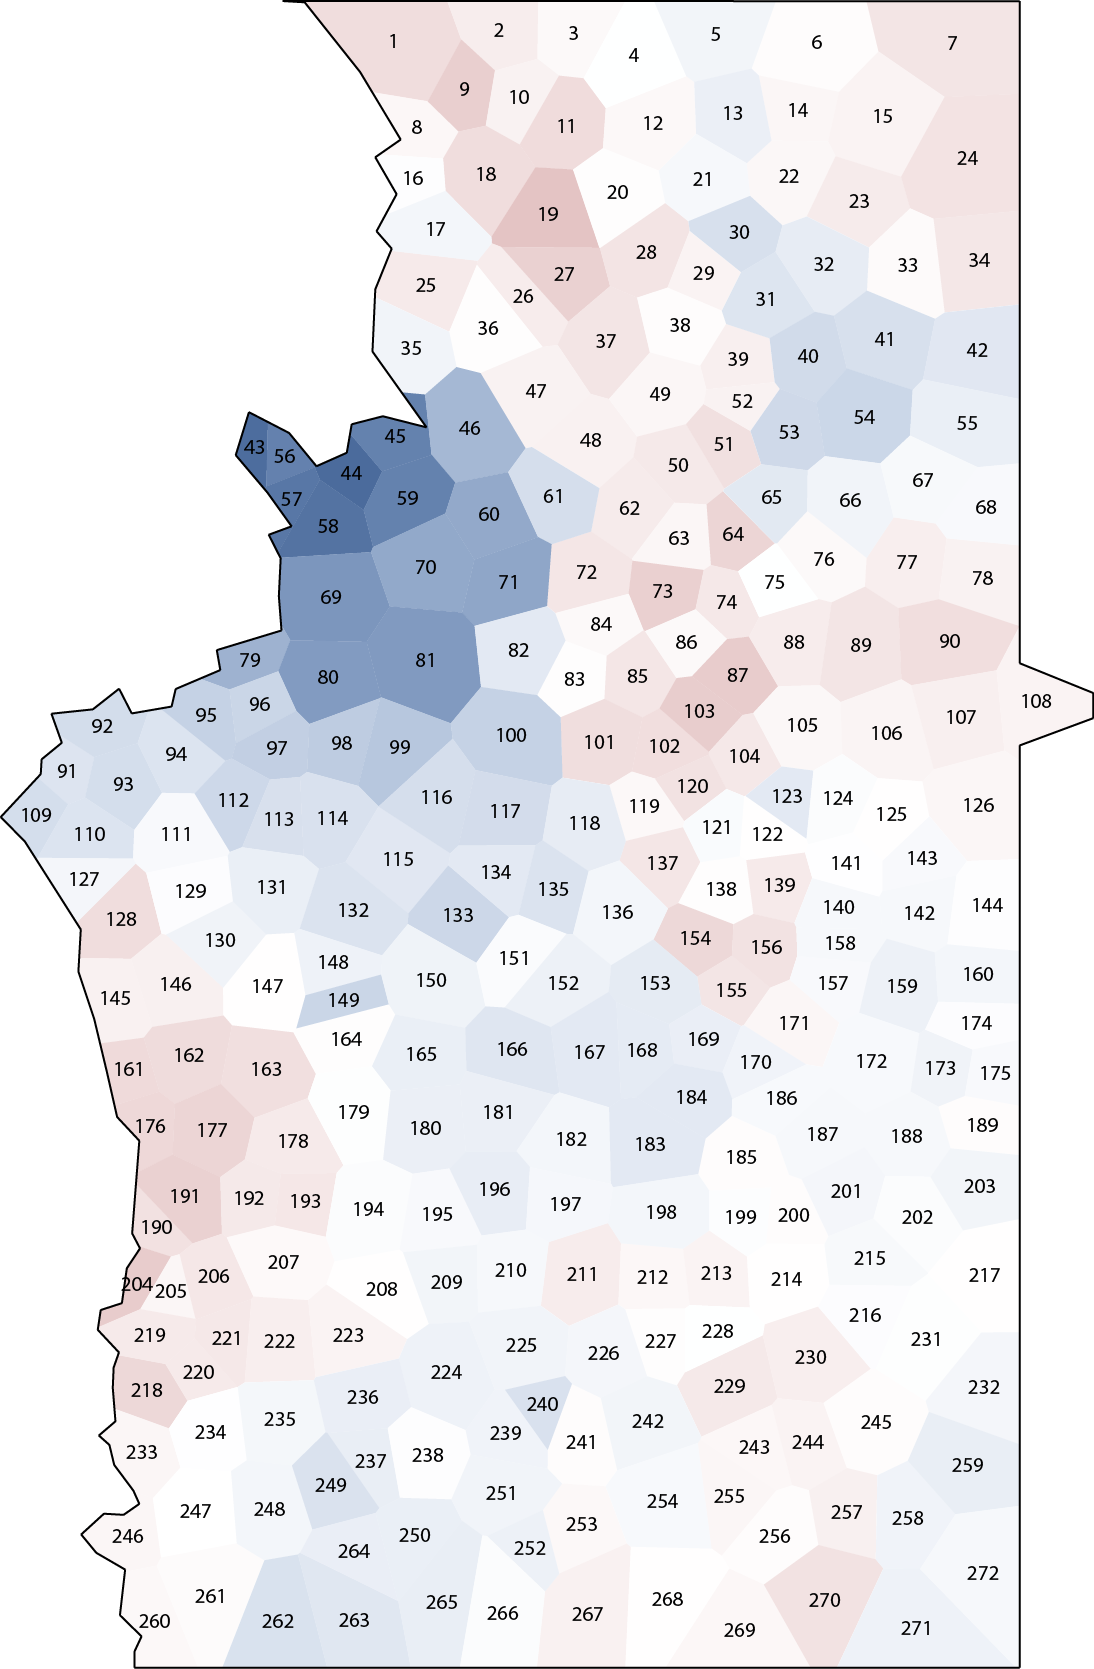
\includegraphics[width=\textwidth]{illustrations/pickl_fig15}
\caption{\figref{fig:15}: Factor 13 (0.71~\%).}
\label{fig:15}
\end{subfigure}   
~
\begin{subfigure}[t]{0.3\textwidth}
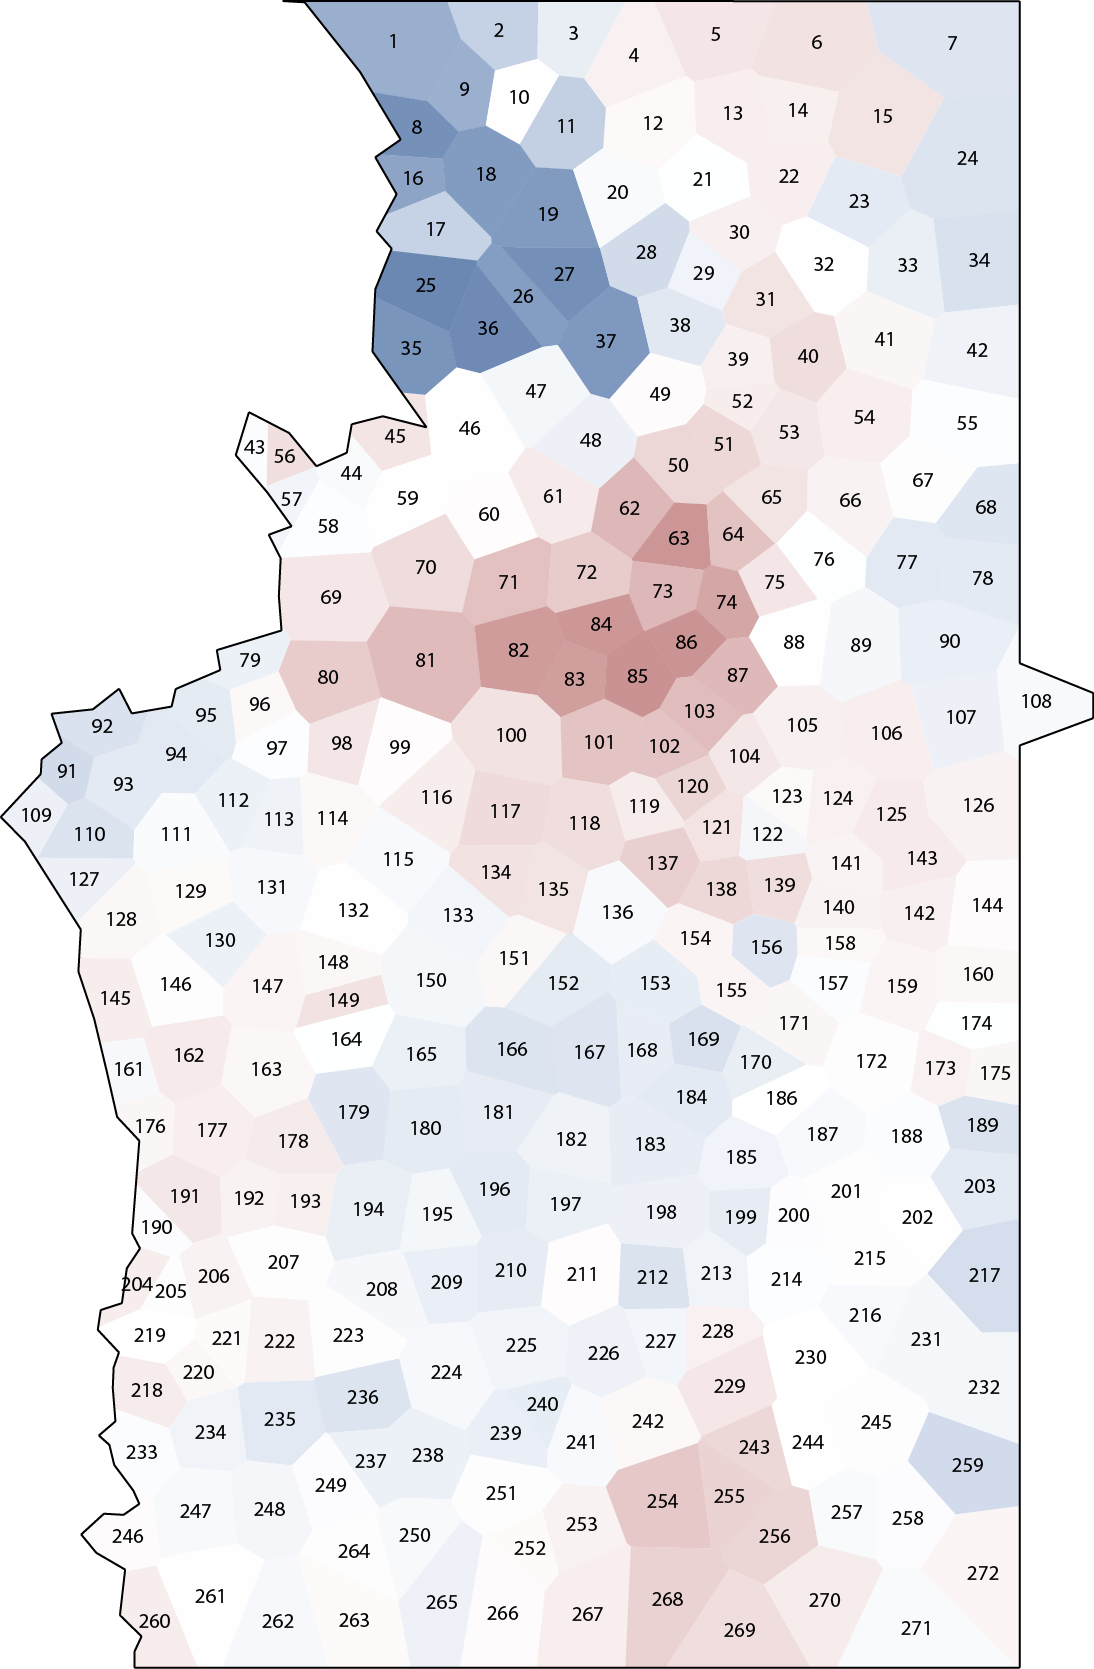
\includegraphics[width=\textwidth]{illustrations/pickl_fig16}
\caption{\figref{fig:16}: Factor 14 (0.62~\%).}
\label{fig:16}
\end{subfigure}  
~
\begin{subfigure}[t]{0.3\textwidth}
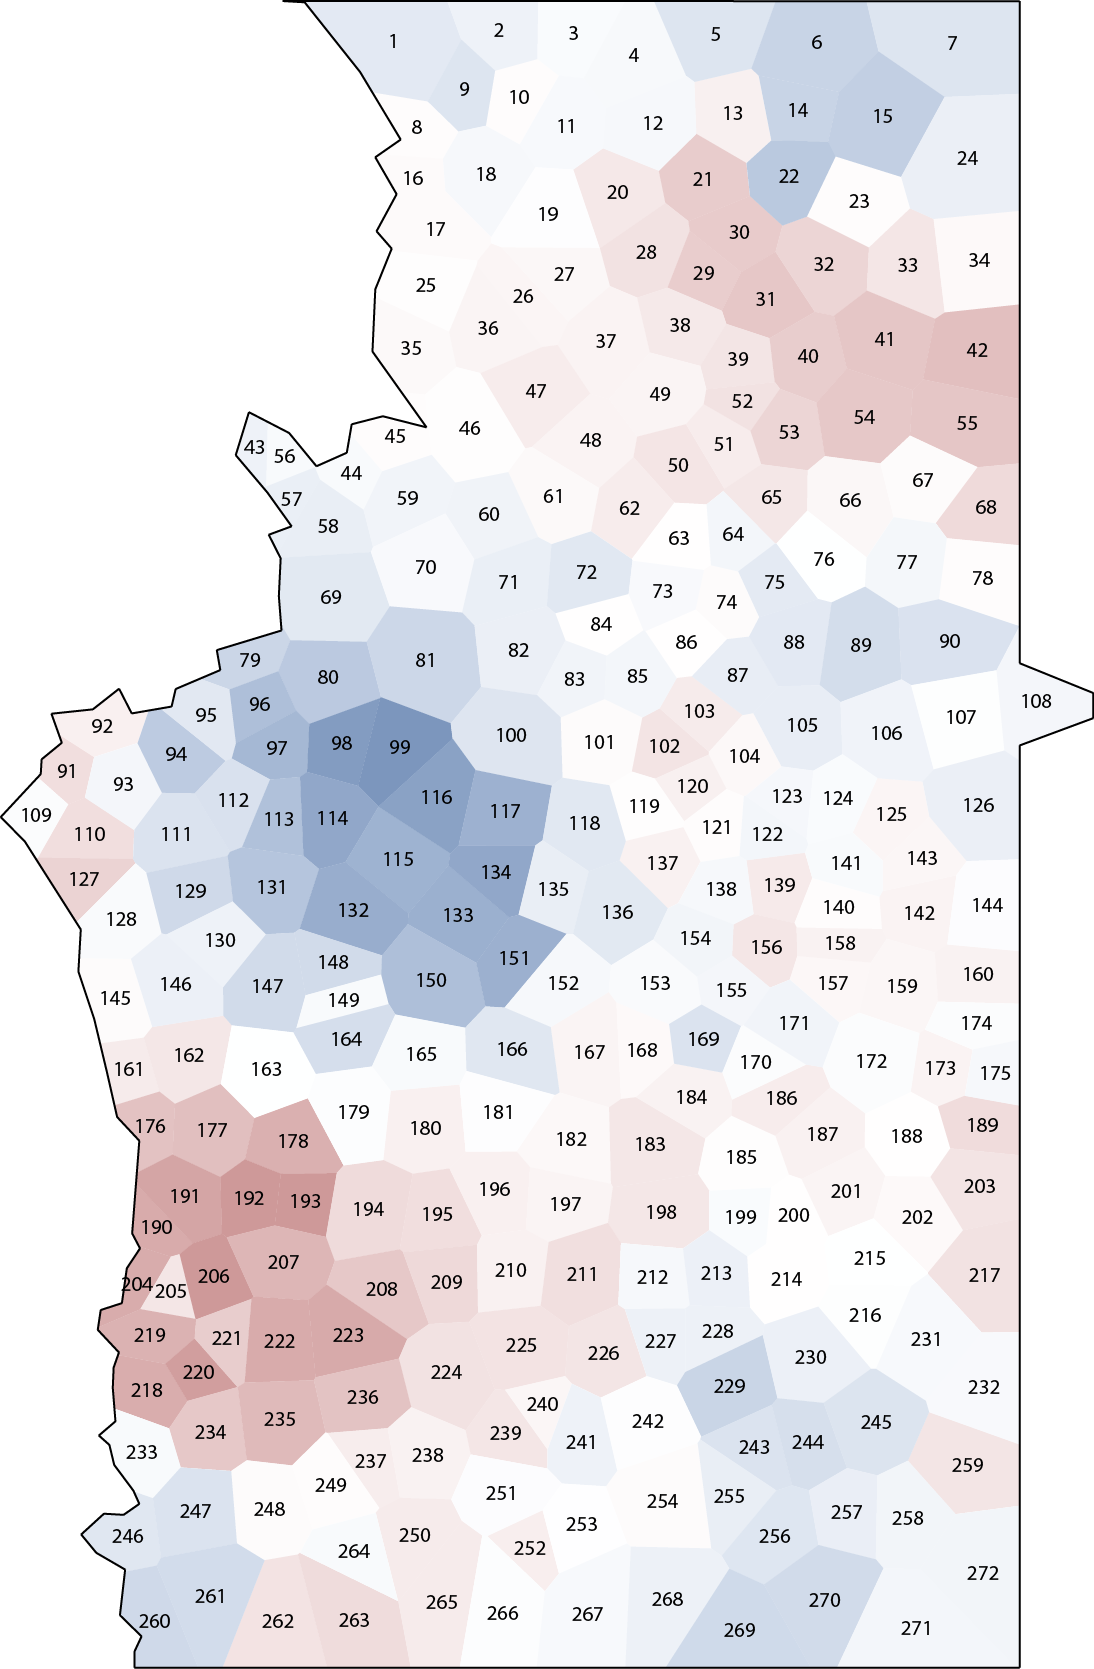
\includegraphics[width=\textwidth]{illustrations/pickl_fig17}
\caption{\figref{fig:17}: Factor 15 (0.60~\%).}
\label{fig:17}
\end{subfigure}
\end{figure}

\begin{figure}
\begin{subfigure}[t]{0.3\textwidth}
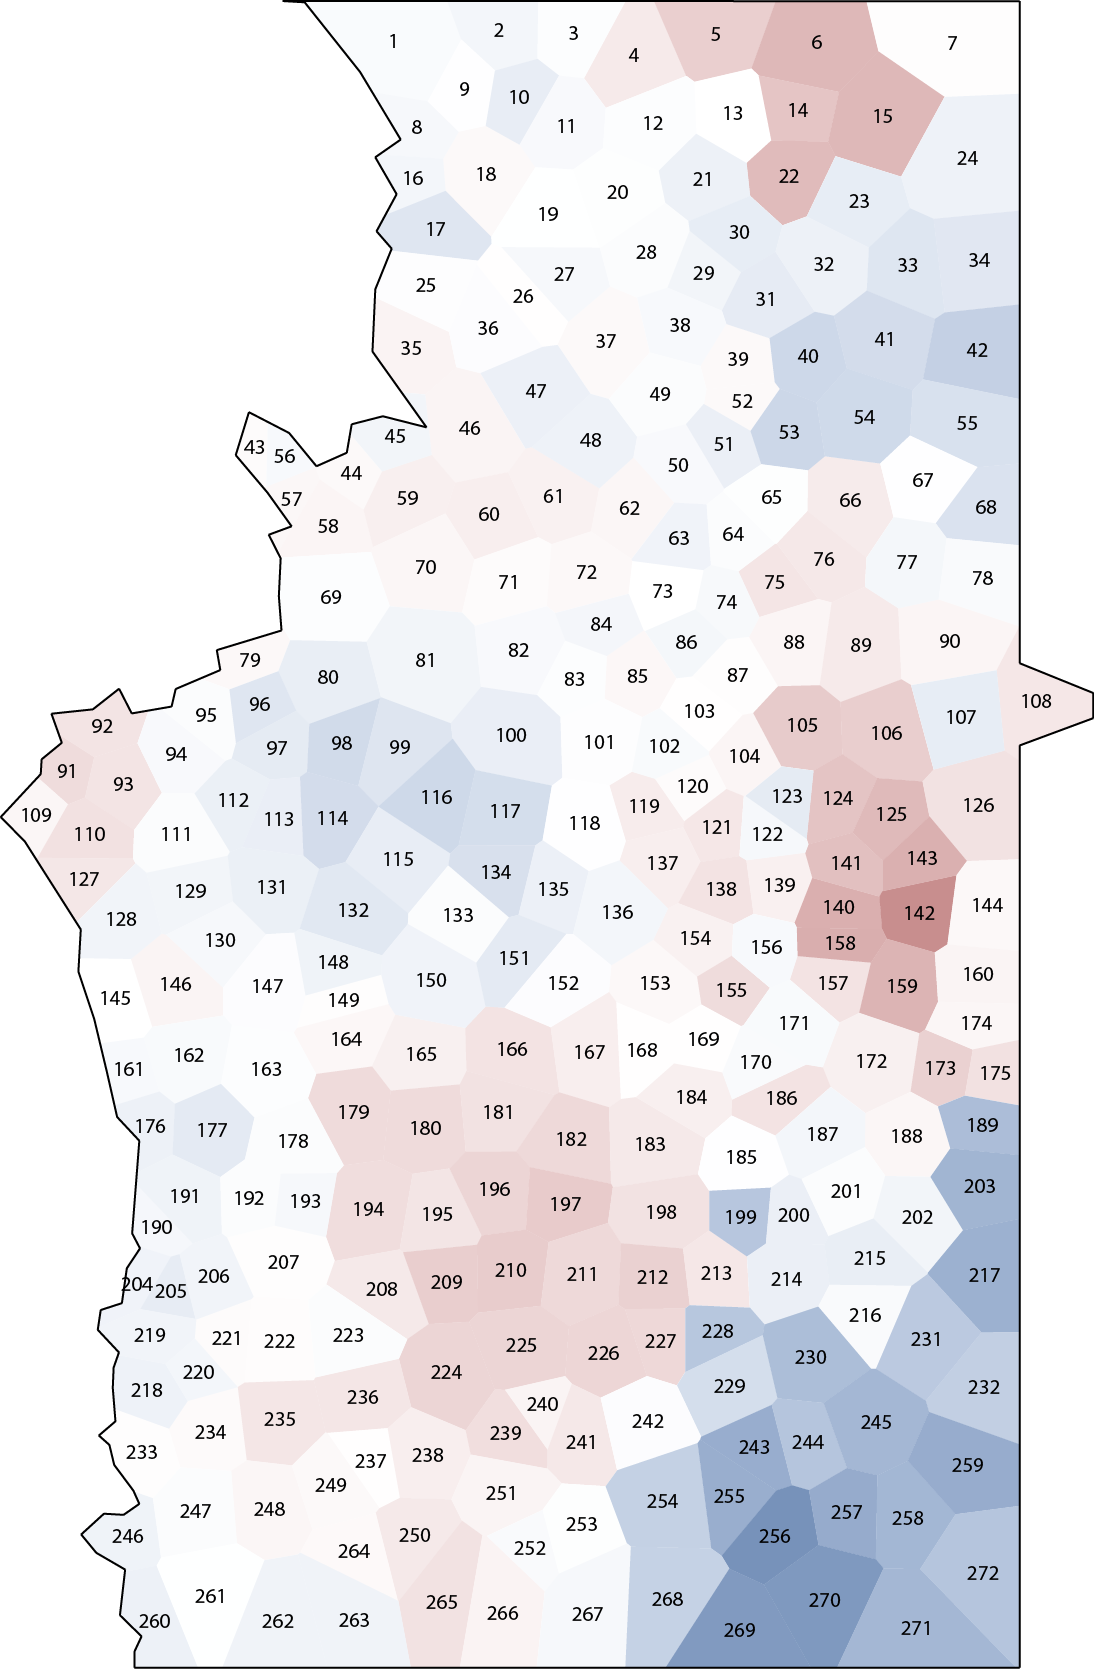
\includegraphics[width=\textwidth]{illustrations/pickl_fig18}
\caption{\figref{fig:18}: Factor 16 (0.51~\%).}
\label{fig:18}
\end{subfigure}
\end{figure}

\section{Conclusion}
It has been demonstrated how prototype theory can be used not only to describe emic, folk ideas of dialects, but also to establish a scholarly, etic notion of dialect areas. Since the two are conceptually similar, they can be compared in a straightforward way in the future to gain insights in the relative importance of individual variants and their evaluation and assessment, e.g. based on their salience.

In this article, it was argued that emic and etic dialect areas alike are best viewed as fuzzy dialect types, which can be described in terms of prototype theory. Dialect types have an unsharp spatial expanse, individual locations exhibiting differential membership values, and are characterised by linguistic features that have individual degrees of relevance for the type.

Following this approach, dialect areas or types are constituted by sets of co-occurring features. It was argued that factor analysis, which was used before in dialectology, is a suitable method for the identification of such sets and thus of dialect types. Its expedience was demonstrated using data from the \textit{Sprachatlas von Bayerisch-Schwaben} (SBS), yielding 16 factors or dialect types. Nine of them are locally dominant within the area of investigation and lead to a classification into fuzzy dialect areas, with broad spans of overlap. Seven are non-dominant, because everywhere, other factors are stronger; they, too, represent meaningful patterns and can be interpreted, as was illustrated using cities’ and towns’ catchment areas.

\section*{Acknowledgments}

This work was supported by the \textit{Deutsche Forschungsgemeinschaft} (DFG), which funded the joint research project \textit{Neue Dialektometrie mit Methoden der stochastischen Bildanalyse} of the Department of German Linguistics (University of Augsburg) and the Institute of Stochastics (Ulm University). My cordial thanks go to all of my colleagues who have contributed to this work, as well as to the editors and reviewers of this volume.

\printbibliography[heading=subbibliography,notkeyword=this]
\end{document}